
\providecommand{\toplevelprefix}{../..}  % necessary for subfile bibliography + figures compilation to work, do not move this after documentclass
\documentclass[../../book-main.tex]{subfiles}
\usepackage[UTF8]{ctex}
\begin{document}

\chapter{熵、扩散与去噪}\label{app:entropy}\label{app:diffusion-denoising}

\begin{quote}
``{\em 无序度或熵随时间的增加,是所谓时间之矢的一个例子,它区分了过去与未来,赋予了时间一个方向。}''

$~$\hfill -- 《时间简史》,史蒂芬·霍金
 \end{quote}
\vspace{5mm}

在本附录中,我们将为\Cref{ch:general-distribution}中提到的几个事实提供证明,这些事实与微分熵以及它在扩散过程下的演化有关。我们将对代表数据源的随机变量(我们称之为\(\vx\))做出以下温和的假设。

\begin{assumption}\label{assumption:entropy_x_compact_support}
    \(\vx\)的支撑集为一个紧集\(\cS \subseteq \R^{D}\),其半径至多为\(R\),即\(R \doteq \sup_{\vxi \in \cS}\norm{\vxi}_{2}\)。
\end{assumption}

特别地,由于欧几里得空间中的紧集是有界的,因此有\(R < \infty\)。我们将统一使用记号\(B_{r}(\vxi) \doteq \{\vu \in \R^{D} \colon \norm{\vxi - \vu}_{2} \leq r\}\)来表示以\(\vxi\)为中心、半径为\(r\)的欧几里得球。在这个意义上,\Cref{assumption:entropy_x_compact_support}意味着\(\cS \subseteq B_{R}(\vzero)\)。

请注意,这个假设在实践中对我们关心的(几乎)所有变量都成立,因为它(通常)是在数据预处理过程中的归一化步骤所施加的。

\section{低维分布的微分熵}\label{sec:low_dim_entropy}

在这个简短的附录中,我们为以下事实提供一个证明。

\begin{theorem}\label{thm:degenerate_entropy_negative_infinity}
    设\(\vx\)为任意满足\Cref{assumption:entropy_x_compact_support}的随机变量,且\(\vx\)的支撑集\(\cS\)的体积为\(0\)。\footnote{严格来说,这意味着\(\cS\)是波莱尔可测的,且其波莱尔测度为\(0\)。} 那么\(h(\vx) = -\infty\)。
\end{theorem}
\begin{proof}
    我们将针对\(\vx\)在\(\cS\)上均匀分布的情况来证明这一点;这种情况抓住了核心思想,而又不过于技术化。其基本思想是对\(\cS\)进行\(\eps\)-增厚,得到\(\cS_{\eps}\),定义为
    \begin{equation}
        S_{\eps} = \bigcup_{\vxi \in \cS}B_{\eps}(\vxi)
    \end{equation}
    如\Cref{fig:entropy_eps_thickening}所示。
    \begin{figure}[th]
        \centering
        \begin{tikzpicture}
            \def\radius{0.2cm} % 定义 epsilon 值
            \def\curve{(0,0) .. controls (1,1.5) and (3,-0.5) .. (4,1)} % 定义曲线 S

            % 沿曲线绘制许多重叠的圆来表示增厚后的 S_eps
            % 使用 decoration 沿路径放置标记(圆)
            \path[decoration={markings, mark=between positions 0 and 1 step 0.02 with {
                    % 在每个标记处填充一个圆;低不透明度以显示重叠
                    \fill[red!30, opacity=0.5, draw=none] (0,0) circle (\radius);
                }}, postaction={decorate}] \curve;

            % 在顶部绘制原始曲线 S,更粗,蓝色
            \draw[blue, thick] \curve node[right, blue] {$\cS$};

            % 在曲线 S 上选择一个示例点 x
            \coordinate (p_on_curve) at (2, 0.5); % 曲线上的一个近似点
            % 为这个 x 绘制特定的球 B_eps(x),颜色稍深/更不透明
            \fill[red!50, opacity=0.7] (p_on_curve) circle (\radius);
            % 标记点 x
            \fill[black] (p_on_curve) circle (1pt) node[below left] {$x$};
            % 添加一个箭头指示这个特定球的半径 epsilon

            % 标记增厚的区域 S_eps,并适当地放置标签
             \node[red, below right] at (3.5, -0.2) {$\cS_{\eps} = \bigcup_{\vxi \in S} B_{\eps}(\vxi)$};

        \end{tikzpicture}
        \caption{曲线\(\cS \subseteq \R^{2}\)的\(\eps\)-增厚\(\cS_\eps\)示意图。}
        \label{fig:entropy_eps_thickening}
    \end{figure}
    我们将处理支撑集为\(\cS_{\eps}\)的随机变量,它是全维的,然后取\(\eps \to 0\)的极限。

    因此,设\(\vx \sim \dUnif(\cS)\),它没有密度\footnote{(相对于\(\R^{D}\)上的波莱尔测度)。},且\(\vx_{\eps} \sim \dUnif(\cS_{\eps})\)。由于\(\cS_{\eps}\)具有正体积,\(\vx_{\eps}\)有一个等于下式的密度\(p_{\eps}\)
    \begin{equation}
        p_{\eps}(\vxi) = \indvar(\vxi \in \cS_{\eps}) \cdot \frac{1}{\volume(\cS_{\eps})}.
    \end{equation}
    由于\(\vx\)没有密度,理解\(h(\vx)\)的方式是通过等式
    \begin{equation}
        h(\vx) = \lim_{\eps \searrow 0}h(\vx_{\eps});
    \end{equation}
    我们将证明后者的极限值为\(-\infty\)。

    确实,根据\(0 \log 0 = 0\)的约定,我们有
    \begin{align}
        h(\vx_{\eps}) 
        &= -\int_{\R^{D}}p_{\eps}(x)\log p_{\eps}(x)\odif{x} \\ 
        &= -\int_{\cS_{\eps}}\frac{1}{\volume(\cS_{\eps})} \log\rp{\frac{1}{\volume(\cS_{\eps})}}\odif{\vxi} \\ 
        &= \frac{\log(\volume(\cS_{\eps}))}{\volume(\cS_{\eps})}\int_{\cS_{\eps}}\odif{\vxi} \\ 
        &= \log(\volume(\cS_{\eps})).
    \end{align}
    由于\(\cS\)是紧集,\(\volume(\cS_{\eps})\)是有限的,并且当\(\eps \searrow 0\)时趋向于\(0\)。\footnote{在\(\cS\)非紧且\(\vx\)在\(\cS\)上非均匀分布的情况下,我们定义一个更精细的\(\vx_{\eps}\)版本,其在\(\vxi\)处的密度在垂直于\(\cS\)和与\(\cS\)对齐的方向上以不同速率变化。这种密度会导致不同的计算,不涉及\(\cS_{\eps}\)的体积,而是涉及一个类似于\(\vx_{\eps}\)所占的有效体积,该体积是有限的,并且当\(\eps \searrow 0\)时趋于零。} 于是
    \begin{equation}
        h(\vx) = \lim_{\eps \searrow 0}h(\vx_{\eps}) = \lim_{\eps \searrow 0}\log(\volume(\cS_{\eps})) = -\infty,
    \end{equation}
    即证。
\end{proof}

上述定理实际上是一组更为著名和重要的结果的推论,这些结果是关于在\(\vx\)的分布满足某些约束条件下,\(\vx\)可能达到的最大熵。我们若不在此处提供这些结果将是一种疏忽,但我们不给出证明;一个合适的参考文献是\cite{poliyanski2024information}。
\begin{theorem}\label{thmx:max_entropy}
    设\(\vx\)是\(\R^{D}\)上的一个随机变量。
    \begin{enumerate}
        \item 如果\(\vx\)的支撑集是一个紧集\(\cS \subseteq \R^{D}\)(即满足\Cref{assumption:entropy_x_compact_support}),那么
        \begin{equation}
            h(\vx) \leq h(\dUnif(\cS)) = \log \volume(\cS).
        \end{equation}
        \item 如果\(\vx\)具有有限协方差,使得对于一个PSD矩阵\(\vSigma \in \PSD(D)\),有\(\Cov(\vx) \preceq \vSigma\)(相对于PSD序,即\(\vSigma - \Cov(\vx)\)是PSD),那么
        \begin{equation}
            h(\vx) \leq h(\dNorm(\vzero, \vSigma)) = \frac{1}{2}\log((2\pi e)^{D}\det\vSigma).
        \end{equation}
        \item 如果\(\vx\)具有有限二阶矩,使得对于一个常数\(a \geq 0\),有\(\Ex\norm{\vx}_{2}^{2} \leq a\),那么
        \begin{equation}
            h(\vx) \leq h\rp{\dNorm\rp{\vzero, \frac{a}{D}\vI}} = \frac{D}{2}\log\frac{2\pi e a}{D}.
        \end{equation}
    \end{enumerate}
\end{theorem}
显然,\Cref{thm:degenerate_entropy_negative_infinity}是\Cref{thmx:max_entropy}.1在\(\volume(\cS) = 0\)时的特例。

\section{扩散与去噪过程}\label{sec:entropy_diffusion}

在正文(\Cref{ch:general-distribution})中,我们考虑了一个随机变量\(\vx\)和一个由\eqref{eq:additive_gaussian_noise_model}定义的随机过程,即:
\begin{equation}\label{eq:app_additive_gaussian_noise_model}
    \vx_{t} = \vx + t\vg, \qquad  \forall t \in [0, T]
\end{equation}
其中\(\vg \sim \dNorm(\vzero, \vI)\)与\(\vx\)独立。

本节的结构如下。在\Cref{sub:diffusion_entropy_increases}中,我们提供一个形式化的定理和清晰的证明,表明在\Cref{eq:app_additive_gaussian_noise_model}下熵是增加的,即\(\odv*{h(\vx_{t})}{t} > 0\)。在\Cref{sub:denoising_entropy_decreases}中,我们提供一个形式化的定理和清晰的证明,表明在\Cref{eq:app_additive_gaussian_noise_model}下,去噪过程中熵是减少的,即对于所有\(s < t\),有\(h(\Ex[\vx_{s} \given \vx_{t}]) < h(\vx_{t})\)。在\Cref{sub:app_diffusion_intermediate_results}中,我们为建立前几小节结论所需的技术性引理提供证明。

在开始之前,我们介绍一些关键的记号。首先,令\(\phi_{t}\)为\(\dNorm(\vzero, t^{2}\vI)\)的密度,即:
\begin{equation}\label{eq:gaussian_noise_time_t}
    \phi_{t}(\vxi) \doteq \frac{1}{(2\pi)^{D/2}t^{D}}\exp\rp{-\frac{\norm{\vxi}_{2}^{2}}{t^{2}}}.
\end{equation}
其次,\(\vx_{t}\)的支撑集是整个\(\R^{D}\),所以它有一个我们记为\(p_{t}\)的\textit{密度}(与正文一致)。一个简单的计算表明
\begin{equation}\label{eq:p_t_representation}
    p_{t}(\vxi) = \Ex[\phi_{t}(\vxi - \vx)],
\end{equation}
并且从这个表示中可以推断出(即,从\Cref{prop:diff_convolution}),\(p_{t}\)在\(\vxi\)上是光滑的(即无限可微),在\(t\)上也是光滑的,并且处处为正。这个事实乍一看相当引人注目:即使对于一个完全不规则的随机变量\(\vx\)(例如,一个没有密度的伯努利随机变量),其高斯平滑对于每个(任意小的)\(t > 0\)都存在一个密度。证明留给精通数学分析的读者作为练习。

然而,我们还需要增加一个关于\(\vx\)分布\textit{光滑性}的假设,这将消除在\(t=0\)附近对于低维分布出现的一些技术性问题。\footnote{因为那时各种量会变得高度不规则,处理它们需要大量的额外分析。}尽管如此,我们期望通过额外的工作,我们的结果在更温和的假设下仍然成立。现在,我们假设:
\begin{assumption}\label{assumption:entropy_x_density}
    \(\vx\)有一个二阶连续可微的密度,记为\(p\)。
\end{assumption}


\subsection{扩散过程熵随时间增加}\label{sub:diffusion_entropy_increases}

在本附录小节中,我们提供\Cref{thm:diffusion_entropy_increases}的证明。为方便起见,我们将其重述如下。

\begin{theorem}[扩散增加熵]\label{thm:diffusion_entropy_increases}
    设\(\vx\)为任意满足\Cref{assumption:entropy_x_compact_support,assumption:entropy_x_density}的随机变量,并设\((\vx_{t})_{t \in [0, T]}\)为随机过程\eqref{eq:app_additive_gaussian_noise_model}。那么
    \begin{equation}\label{eq:diffusion_entropy_increases}
        h(\vx_{s}) < h(\vx_{t}), \qquad \forall s, t \colon 0 \leq s < t \leq T.
    \end{equation}
\end{theorem}
\begin{proof}
    在开始之前,让我们先解决一个学究式的问题:\eqref{eq:diffusion_entropy_increases}中的不等式在何时有意义?我们将在\Cref{lem:diffusion_entropy_exists}中证明,在我们的假设下,微分熵是良定义的,永远不为\(+\infty\),并且对于\(t > 0\)是有限的,因此\eqref{eq:diffusion_entropy_increases}中的(严格)不等式是有意义的。

    抛开学究式的讨论,此证明的关键在于表明\(\vx_{t}\)的密度\(p_{t}\)满足一个特定的偏微分方程,该方程与\textit{热传导方程}非常相似。热传导方程是一个著名的偏微分方程,描述了热量在空间中的扩散。这在直觉上是合理的,并描绘了一幅生动的画面:随着时间\(t\)的增加,来自原始(可能高度集中的)\(\vx\)的概率像热量从真空中的热源辐射一样,散布到整个\(\R^{D}\)空间。
    
    这类关于\(p_{t}\)的偏微分方程,对于更一般的随机过程被称为\textit{福克-普朗克方程},是非常强大的工具,因为它们允许我们用\(p_{t}\)的瞬时空间导数来描述其瞬时时间导数,反之亦然,从而为\(p_{t}\)的正则性和动力学提供了简洁的描述。一旦我们得到了\(p_{t}\)的动力学方程,我们就可以利用这个系统得到另一个描述\(h(\vx_{t})\)动力学的方程,毕竟\(h(\vx_{t})\)只是\(p_{t}\)的一个泛函。

    该偏微分方程的描述涉及一个称为拉普拉斯算子\(\Delta\)的数学对象。回想一下你在多元微积分课上学到的,作用于一个时间上可微、空间上二阶可微的函数\(f \colon (0, T) \times \R^{D} \to \R\)的拉普拉斯算子由下式给出
    \begin{equation}
        \Delta f_{t}(\vxi) = \tr(\nabla^{2}f_{t}(\vxi)) = \sum_{i = 1}^{D}\pdv[order=2]{f_{t}}{\xi_{i}}(\vxi).
    \end{equation}
    
    也就是说,通过使用\(p_{t}\)的积分表示并在积分号下求导,我们可以计算出\(p_{t}\)的导数(这在\Cref{prop:p_t_derivatives}中完成),并观察到\(p_{t}\)满足类似热传导的偏微分方程
    \begin{equation}
        \pdv{p_{t}}{t}(\vxi) = t\Delta p_{t}(\vxi).
    \end{equation}
    然后为了找到\(h(\vx_{t})\)的动力学,我们可以再次使用\Cref{prop:dutis}以及类似热传导的偏微分方程来得到
    \begin{align}
        \odv*{h(\vx_{t})}{t}
        &= -\odv*{\int_{\R^{D}}p_{t}(\vxi)\log p_{t}(\vxi)\odif{\vxi}}{t} \\
        &= -\int_{\R^{D}}\pdv*{\bs{p_{t}(\vxi)\log p_{t}(\vxi)}}{t}\odif{\vxi} \\
        &= -\int_{\R^{D}}\pdv{p_{t}}{t}(\vxi)[1 + \log p_{t}(\vxi)]\odif{\vxi} \\
        &= -t\int_{\R^{D}}\Delta p_{t}(\vxi)[1 + \log p_{t}(\vxi)]\odif{\vxi}.
    \end{align}
    通过使用一个稍微复杂的分部积分论证(\Cref{lem:diffusion_ibp}),我们得到
    \begin{align}
        \odv*{h(\vx_{t})}{t}
        &= t\int_{\R^{D}}\ip{\nabla \log p_{t}(\vxi)}{\nabla p_{t}(\vxi)}\odif{\vxi} \\
        &= t\int_{\R^{D}}\frac{\norm{\nabla p_{t}(\vxi)}_{2}^{2}}{p_{t}(\vxi)}\odif{\vxi} \\
        &> 0
    \end{align}
    其中最后一行严格不等式成立,因为若不等式不成立,\(\nabla p_{t}(\vxi)\)需要几乎处处为零(即,除了可能在一个零体积集合上),但这将意味着\(p_{t}\)几乎处处为常数,这与\(p_{t}\)是一个密度的事实相矛盾。

    为了完成证明,我们只需使用微积分基本定理
    \begin{equation}
        h(\vx_{t}) = h(\vx_{s}) + \int_{s}^{t}\odv*{h(\vx_{u})}{u}\odif{u} > h(\vx_{s}),
    \end{equation}
    这就证明了我们的论断。(请注意,当\(h(\vx_{s}) = -\infty\)时,这个式子没有意义,这种情况只可能在\(s=0\)且\(h(\vx)=-\infty\)时发生,但在这种情况下\(h(\vx_{t}) > -\infty\),所以该论断无论如何都是不言自明的。)
\end{proof}

\subsection{去噪过程熵随时间减少}\label{sub:denoising_entropy_decreases}

回想一下,在\Cref{sub:intro_diffusion_denoising}中,我们从随机变量\(\vx_{T}\)开始,并使用如下形式的迭代来对其进行去噪
\begin{equation}\label{eq:app_denoising_iteration}
    \hat{\vx}_{s} \doteq \Ex[\vx_{s} \mid \vx_{t} = \hat{\vx}_{t}] = \frac{s}{t}\hat{\vx}_{t} + \bp{1 - \frac{s}{t}}\bar{\vx}^{\ast}(t, \hat{\vx}_{t}).
\end{equation}
对于\(s, t \in \{t_{0}, t_{1}, \dots, t_{L}\}\)且满足\(s < t\)和\(\vx_{T} = \hat{\vx}_{T}\)。我们希望证明\(h(\hat{\vx}_{s}) < h(\hat{\vx}_{t})\),从而表明去噪过程确实减少了熵。

在进行证明之前,我们对问题陈述做几点说明。首先,Tweedie公式\eqref{eq:tweedie}表明
\begin{equation}
    \bar{\vx}^{\ast}(t, \vx_{t}) = \vx_{t} + t^{2}\nabla p_{t}(\vx_{t}),
\end{equation}
这将从时间\(t\)到时间\(0\)的完整去噪步骤比作在\(\vx_{t}\)的对数密度上进行的一个梯度步。我们能否为\eqref{eq:app_denoising_iteration}中从时间\(t\)到时间\(s\)的完整去噪步骤得到类似的结果?事实证明,我们确实可以,而且非常简单。通过使用\eqref{eq:app_denoising_iteration}和Tweedie公式\eqref{eq:tweedie},我们得到
\begin{equation}\label{eq:app_denoising_iteration_score}
    \Ex[\vx_{s} \mid \vx_{t}] = \frac{s}{t}\vx_{t} + \bp{1 - \frac{s}{t}}\bp{\vx_{t} + t^{2}\nabla_{\vx_{t}}\log p_{t}(\vx_{t})} = \vx_{t} + \bp{1 - \frac{s}{t}}t^{2}\nabla_{\vx_{t}}\log p_{t}(\vx_{t}).
\end{equation}
所以这个迭代去噪步骤又是在扰动后的对数密度\(\log p_{t}\)上的一个梯度步,步长有所缩减。特别地,这一步可以看作是通过\textit{分数函数向量场}对随机变量\(\vx_{t}\)的分布进行扰动,这暗示了与随机微分方程(SDEs)和扩散模型理论\cite{song2020score}的联系。实际上,可以使用这种强大的工具和极限论证来推导以下结果\Cref{thm:conditioning_reduces_entropy}的证明(例如,遵循\cite{DBLP:conf/iclr/ChenC0LSZ23}的阐述中的技术方法)。我们将在这里给出一个更简单的证明,它只使用基本工具,从而阐明通过去噪减少熵过程背后的一些关键量。另一方面,由于\Cref{thm:conditioning_reduces_entropy}中的去噪过程并\textit{不}完全对应于生成观测值\(\vx_{t}\)的加噪过程的\textit{逆}过程,我们将需要处理一些略带技术性的计算。\footnote{对于熟悉扩散模型的读者,我们这里指的是时间反向的前向过程与由\Cref{thm:conditioning_reduces_entropy}定义的过程生成的迭代序列不一致。这些过程在某个极限下是一致的,即当\Cref{thm:conditioning_reduces_entropy}的无限多步以无限小的噪声水平在每一步添加时;对于一般的有限步,无论我们工具的复杂程度如何,我们都必须引入一些近似。}

我们想要证明\(h(\Ex[\vx_{s} \mid \vx_{t}]) < h(\vx_{t})\),即,形式化地:
\begin{theorem}\label{thm:conditioning_reduces_entropy}
    设\(\vx\)为任意满足\Cref{assumption:entropy_x_compact_support,assumption:entropy_x_density}的随机变量,并设\((\vx_{t})_{t \in [0, T]}\)为随机过程\eqref{eq:app_additive_gaussian_noise_model}。那么
    \begin{equation}
        h(\Ex[\vx_{s} \mid \vx_{t}]) < h(\vx_{t}), \qquad \forall s, t \in [0, T] \colon \quad 0 < t \leq \frac{R}{\sqrt{2D}}, \quad 0 \leq s  < t\cdot\min\bc{1, \frac{R^{2}/D - 2t^{2}}{R^{2}/D - t^{2}}}.
    \end{equation}
\end{theorem}
\begin{proof}
    此证明使用两个主要思想:
    \begin{enumerate}
        \item 首先,使用变量替换公式写出\(\Ex[\vx_{s} \mid \vx_{t}]\)的密度。
        \item 其次,对该密度进行界定以控制熵。
    \end{enumerate}
    变量替换的合理性由\Cref{cor:gribonval_A2}保证,该结论最初在\cite{Gribonval2011-pf}中推导得出。

    我们现在来执行这些思想。从\Cref{cor:gribonval_A2}可知,定义为\(\bar{\vx}(\vxi) \doteq \Ex[\vx_{s} \given \vx_{t} = \vxi]\)的函数\(\bar{\vx}\)是可微的、单射的,因此在其值域上是可逆的,我们此后将其值域记为\(\cX \subseteq \R^{D}\)。我们将其逆记为\(\bar{\vx}^{-1}\)。使用变量替换公式,\(\bar{\vx}(\vx_{t})\)的密度\(\bar{p}\)由下式给出
    \begin{equation}
        \bar{p}(\vxi) \doteq \frac{(p_{t} \circ \bar{\vx}^{-1})(\vxi)}{\det(\bar{\vx}^{\prime}(\bar{\vx}^{-1}(\vxi)))},
    \end{equation}
    其中(回想一下,从\Cref{app:optimization}可知)\(\bar{\vx}^{\prime}\)是\(\bar{\vx}\)的雅可比矩阵。由于从\Cref{lem:gribonval_A1}我们知道\(\bar{\vx}^{\prime}\)是一个正定矩阵,其行列式为正,因此整个密度为正。于是有
    \begin{align}
        h(\bar{\vx}(\vx_{t}))
        &= -\int_{\cX}\frac{(p_{t} \circ \bar{\vx}^{-1})(\vxi)}{\det(\bar{\vx}^{\prime}(\bar{\vx}^{-1}(\vxi)))} \log \frac{(p_{t} \circ \bar{\vx}^{-1})(\vxi)}{\det(\bar{\vx}^{\prime}(\bar{\vx}^{-1}(\vxi)))} \odif{\vxi} \\ 
        &= -\int_{\cX}\frac{(p_{t} \circ \bar{\vx}^{-1})(\vxi)}{\det(\bar{\vx}^{\prime}(\bar{\vx}^{-1}(\vxi)))} \log((p_{t} \circ \bar{\vx}^{-1})(\vxi))\odif{\vxi} \\ 
        &\qquad + \int_{\cX}\frac{(p_{t} \circ \bar{\vx}^{-1})(\vxi)}{\det(\bar{\vx}^{\prime}(\bar{\vx}^{-1}(\vxi)))}\logdet\rp{\bar{\vx}^{\prime}(\bar{\vx}^{-1}(\vxi))}\odif{\vxi} \\ 
        &= -\int_{\R^{D}}p_{t}(\vxi)\log p_{t}(\vxi)\odif{\vxi} + \int_{\cX}\frac{(p_{t} \circ \bar{\vx}^{-1})(\vxi)}{\det(\bar{\vx}^{\prime}(\bar{\vx}^{-1}(\vxi)))}\logdet\rp{\bar{\vx}^{\prime}(\bar{\vx}^{-1}(\vxi))}\odif{\vxi} \\ 
        &= h(\vx_{t}) - \int_{\cX}\frac{(p_{t} \circ \bar{\vx}^{-1})(\vxi)}{\det(\bar{\vx}^{\prime}(\bar{\vx}^{-1}(\vxi)))}\log\rp{\frac{1}{\det(\bar{\vx}^{\prime}(\bar{\vx}^{-1}(\vxi)))}}\odif{\vxi}.
    \end{align}
    我们将研究最后一项(包括负号),并证明其为负。

    根据凹性,对于每个\(x \geq 0\),有\(-x\log x \leq 1 - x\)。因此
    \begin{align}
        h(\bar{\vx}(\vx_{t})) - h(\vx_{t})
        &= - \int_{\cX}\frac{(p_{t} \circ \bar{\vx}^{-1})(\vxi)}{\det(\bar{\vx}^{\prime}(\bar{\vx}^{-1}(\vxi)))}\log\rp{\frac{1}{\det(\bar{\vx}^{\prime}(\bar{\vx}^{-1}(\vxi)))}}\odif{\vxi} \\ 
        &\leq  \int_{\cX}(p_{t} \circ \bar{\vx}^{-1})(\vxi)\cdot \bp{1 - \frac{1}{\det(\bar{\vx}^{\prime}(\bar{\vx}^{-1}(\vxi)))}}\odif{\vxi} \\ 
        &= \int_{\cX}(p_{t} \circ \bar{\vx}^{-1})(\vxi)\odif{\vxi} - \int_{\cX}\frac{(p_{t} \circ \bar{\vx}^{-1})(\vxi)}{\det(\bar{\vx}^{\prime}(\bar{\vx}^{-1}(\vxi)))}\odif{\vxi} \\
        &= \int_{\R^{D}}p_{t}(\vxi)\det\rp{\bar{\vx}^{\prime}(\bar{\vx}^{-1}(\vxi))}\odif{\vxi} - \int_{\cX}\bar{p}(\vxi)\odif{\vxi} \\
        &= \int_{\R^{D}}p_{t}(\vxi)\det\rp{\vI + \bp{1 - \frac{s}{t}}t^{2}\nabla^{2}\log p_{t}(\vxi)}\odif{\vxi} - 1.
    \end{align}
    现在,通过对特征值使用算术-几何平均不等式(AM-GM),我们对于任何对称正定矩阵\(\vM \in \PSD(D)\)有如下界
    \begin{equation}
        \det(\vM)^{1/D} = \prod_{i = 1}^{D}\lambda_{i}(\vM)^{1/D} \leq \frac{\sum_{i = 1}^{D}\lambda_{i}(\vM)}{D} = \frac{\tr(\vM)}{D},
    \end{equation}
    我们可以将其应用于上述表达式并得到
    \begin{align}
        &\int_{\R^{D}}p_{t}(\vxi)\det\rp{\vI + \bp{1 - \frac{s}{t}}t^{2}\nabla^{2}\log p_{t}(\vxi)}\odif{\vxi} \\
        &\leq \int_{\R^{D}} p_{t}(\vxi) \tr\rp{\frac{1}{D}\bs{\vI + \bp{1 - \frac{s}{t}}t^{2}\nabla^{2}\log p_{t}(\vxi)}}^{D}\odif{\vxi} \\
        &= \int_{\R^{D}} p_{t}(\vxi)\bp{1 + \frac{\bp{1 - \frac{s}{t}}t^{2}}{D}\tr(\nabla^{2}\log p_{t}(\vxi))}^{D}\odif{\vxi} \\
        &= \int_{\R^{D}} p_{t}(\vxi)\bp{1 + \frac{\bp{1 - \frac{s}{t}}t^{2}}{D}\Delta \log p_{t}(\vxi)}^{D}\odif{\vxi}.
    \end{align}
    从\Cref{lem:app_diffusion_laplacian_control}可知,(其中,回想一下,\(R\)是\(\vx\)支撑集的半径,如\Cref{assumption:entropy_x_compact_support}中所定义)
    \begin{equation}
        \abs{\Delta \log p_{t}(\vxi)} \leq \max\rp{\frac{D}{t^{2}}, \abs*{\frac{R^{2}}{t^{4}} - \frac{D}{t^{2}}}} =: U_{t}.
    \end{equation}
    于是有
    \begin{equation}
        -\frac{\bp{1 - \frac{s}{t}}t^{2}}{D}U_{t} \leq \frac{\bp{1 - \frac{s}{t}}t^{2}}{D}\Delta \log p_{t}(\vxi) \leq \frac{\bp{1 - \frac{s}{t}}t^{2}}{D}U_{t}.
    \end{equation}
    同时,函数\(x \mapsto (1 + x)^{D}\)在\([-1, \infty)\)上是凸的,因此对于
    \(-(1-s/t)t^{2}U_{t}/D \leq x \leq (1-s/t)t^{2}U_{t}/D\)我们有
    \begin{align}
        (1 + x)^{d} 
        &\leq \bp{1 - \frac{\bp{1 - \frac{s}{t}}t^{2}U_{t}}{D}}^{D} + \underbrace{\bs{\bp{1 + \frac{\bp{1 - \frac{s}{t}}t^{2}U_{t}}{D}}^{D} - \bp{1 - \frac{\bp{1 - \frac{s}{t}}t^{2}U_{t}}{D}}^{D}}}_{M(s, t, D)}x \\ 
        &\leq 1 + M(s, t, D)x.
    \end{align}
    这里\(M(s, t, D) > 0\)因为\(U_{t} > 0\)。在上述界中,我们需要验证\(x\)的下界\(\geq -1\)。确实,
    \begin{align}
        -\frac{\bp{1 - \frac{s}{t}}t^{2}}{D}U_{t}
        &= -\frac{\bp{1 - \frac{s}{t}}t^{2}}{D}\max\rp{\frac{D}{t^{2}}, \abs*{\frac{R^{2}}{t^{4}} - \frac{D}{t^{2}}}} \\ 
        &= -\bp{1 - \frac{s}{t}}\max\rp{1, \abs*{\frac{R^{2}}{Dt^{2}} - 1}}
    \end{align}
    注意到,这\(\geq -1\)当且仅当\(\bp{1 - \frac{s}{t}}\cdot\bp{\frac{R^{2}}{Dt^{2}} - 1} \geq 1\),即\(0 < t < R/\sqrt{2D}\)且\(0 \leq s \leq t\cdot\frac{R^{2}/D - 2t^{2}}{R^{2}/D - t^{2}}\),这由假设所保证。
    
    应用这个界,我们得到
    \begin{align}
        &\int_{\R^{D}} p_{t}(\vxi)\bp{1 + \frac{\bp{1 - \frac{s}{t}}t^{2}}{D}\Delta \log p_{t}(\vxi)}^{D}\odif{\vxi} \\ 
        &\leq \int_{\R^{D}}p_{t}(\vxi)\bp{1 + M(s, t, D)\Delta \log p_{t}(\vxi)}\odif{\vxi} \\
        &= 1 + M(s, t, D)\int_{\R^{D}}p_{t}(\vxi)\Delta \log p_{t}(\vxi)\odif{\vxi} \\
        &= 1 - M(s, t, D)\int_{\R^{D}}\ip{\nabla p_{t}(\vxi)}{\nabla\log p_{t}(\vxi)}\odif{\vxi} \\
        &= 1 - M(s, t, D)\int_{\R^{D}}\frac{\norm{\nabla p_{t}(\vxi)}_{2}^{2}}{p_{t}(\vxi)}\odif{\vxi},
    \end{align}
    其中最后几行与\Cref{thm:diffusion_entropy_increases}的证明中相同。将此结果与我们之前的估计相结合,
    \begin{equation}
        h(\bar{\vx}(\vx_{t})) - h(\vx_{t}) \leq - M(s, t, D)\int_{\R^{D}}\frac{\norm{\nabla p_{t}(\vxi)}_{2}^{2}}{p_{t}(\vxi)}\odif{\vxi} < 0
    \end{equation}
    其中不等式是严格的,论证与\Cref{thm:diffusion_entropy_increases}中相同。
\end{proof}

请注意,\(s\)和\(t\)的界依赖于数据分布的半径\(R\),不像\Cref{thm:diffusion_entropy_increases}中的界那样具有普遍性。这个结果实际上在以下意义上是“足够通用”的。注意,如果\(\vx\)有一个二阶连续可微的密度,其支撑集是以\(\vzero\)为中心、半径为\(R\)的球,那么对于\(2R\)、\(3R\)等,即对于任何半径为\(R^{\prime} > R\)的球,它也成立。因此,获得适当去噪保证的一个策略是:固定数据维度\(D\)和离散化方案,然后在分析中将数据半径\(R\)设置得非常大,以使每个去噪步骤都满足\Cref{thm:conditioning_reduces_entropy}中给出的熵减少的要求。这样,去噪过程的每一步确实会如期望的那样减少熵。

 
\subsection{技术性引理与中间结果}\label{sub:app_diffusion_intermediate_results}

在本小节中,我们介绍为我们两个主要概念性定理提供支持的技术性结果。我们的表述将或多或少遵循数学的标准;我们将首先从更高层次的结果开始,然后逐渐回到更具增量性的结果。高层次的结果将使用增量性的结果,这样我们就得到了一个易于阅读的结果依赖顺序:没有结果依赖于它之前的结果。互不依赖的结果通常按照它们在上述两个证明中出现的顺序排列。


\subsubsection{微分熵的有限性}

我们首先证明熵在随机过程中存在且是有限的。

\begin{lemma}\label{lem:diffusion_entropy_exists}
    设\(\vx\)为任意随机变量,并设\((\vx_{t})_{t \in [0, T]}\)为随机过程\eqref{eq:app_additive_gaussian_noise_model}。
    \begin{enumerate}
        \item 对于\(t > 0\),微分熵\(h(\vx_{t})\)存在且\(> -\infty\)。
        \item 如果\(\vx\)还满足\Cref{assumption:entropy_x_compact_support},那么\(h(\vx) < \infty\)且\(h(\vx_{t})\ < \infty\)。
    \end{enumerate}
\end{lemma}
\begin{proof}
    为证明\Cref{lem:diffusion_entropy_exists}.1,我们使用一个经典但繁琐的分析论证。由于\(\vx_{t}\)有密度,我们可以写出
    \begin{equation}
        h(\vx_{t}) = -\int_{\R^{D}}p_{t}(\vxi)\log p_{t}(\vxi) \odif{\vxi}.
    \end{equation}
    相应地,令\(g \colon \R^{D} \to \R\)定义为
    \begin{equation}
        g(\vxi) \doteq -p_{t}(\vxi)\log p_{t}(\vxi) \implies h(\vx_{t}) = \int_{\R^{D}}g(\vxi)\odif{\vxi}.
    \end{equation}
    按照分析学中界定积分值的常规方法,定义
    \begin{equation}
        g_{+}(\vxi) \doteq \max(g(\vxi), 0), \quad g_{-}(\vxi) \doteq \max(-g(\vxi), 0) \quad \implies \quad g = g_{+} - g_{-}\quad \text{and} \quad g_{+}, g_{-} \geq 0.
    \end{equation}
    那么
    \begin{equation}
        h(\vx_{t}) = \int_{\R^{D}}g_{+}(\vxi)\odif{\vxi} - \int_{\R^{D}}g_{-}(\vxi)\odif{\vxi},
    \end{equation}
    并且由于被积函数非负,这两个积分都保证是非负的。
    
    为了证明\(h(\vx_{t})\)是良定义的,我们需要证明\(\int_{\R^{D}}g_{+}(\vxi)\odif{\vxi} < \infty\)或\(\int_{\R^{D}}g_{-}(\vxi) \odif{\vxi} < \infty\)。为了证明\(h(\vx_{t}) > -\infty\),只需证明\(\int_{\R^{D}}g_{-}(\vxi)\odif{\vxi} < \infty\)即可。为了界定\(g_{-}\)的积分,我们需要理解\(g_{-}\)这个量,即,我们想刻画\(g\)何时为负。
    \begin{equation}
        g(\vxi) \leq 0 \iff p_{t}(\vxi)\log p_{t}(\vxi) \geq 0 \iff \log p_{t}(\vxi) \geq 0 \iff p_{t}(\vxi) \geq 1.
    \end{equation}
    因此,我们有
    \begin{equation}
        g_{-}(\vxi) = \indvar(p_{t}(\vxi) \geq 1)\cdot (-g(\vxi)) = \indvar(p_{t}(\vxi) \geq 1)p_{t}(\vxi)\log p_{t}(\vxi).
    \end{equation}
    为了界定\(g_{-}(\vxi)\)的积分,我们需要证明\(p_{t}\)“不太集中”,即\(p_{t}\)不太大。为了证明这一点,在这种情况下,我们很幸运能够直接界定函数\(g_{-}(\vxi)\)本身。也就是说,注意到
    \begin{equation}
        \max_{\vxi \in \R^{D}}\phi_{t}(\vxi - \vx) = \phi_{t}(\vzero) = \frac{1}{(2\pi)^{D/2}t^{D}} =: C_{t}.
    \end{equation}
    当\(t \to 0\)时它会趋于无穷,但对于所有有限的\(t\)都是有限的。因此
    \begin{equation}
        p_{t}(\vxi) = \Ex \phi_{t}(\vxi - \vx) \leq \Ex C_{t} = C_{t}.
    \end{equation}
    现在有两种情况。
    \begin{itemize}
        \item 如果\(C_{t} < 1\),那么\(p_{t}(\vxi) < 1\),所以指示函数永远不为\(1\),因此\(g_{-}\)恒等于\(0\),其积分也为\(0\)。
        \item 如果\(C_{t} \geq 1\),那么\(\log C_{t} \geq 0\),所以由于对数函数是单调递增的,
        \begin{align}
            \int_{\R^{D}}g_{-}(\vxi)\odif{\vxi}
            &= \int_{\R^{D}}\indvar(p_{t}(\vxi) \geq 1)p_{t}(\vxi)\log p_{t}(\vxi)\odif{\vxi}  \\ 
            &= \Ex[\indvar(p_{t}(\vx_{t}) \geq 1)\log p_{t}(\vx_{t})]  \\ 
            &\leq \Ex[\indvar(p_{t}(\vx_{t}) \geq 1) \log C_{t}] \\ 
            &= \Pr[p_{t}(\vx_{t}) \geq 1]\log C_{t}.
        \end{align}
    \end{itemize}
    因此我们有\(\int_{\R^{D}}g_{-}(\vxi)\odif{\vxi} < \infty\),所以微分熵\(h(\vx_{t})\)存在且\(> -\infty\)。

    为证明\Cref{lem:diffusion_entropy_exists}.2,假设\Cref{assumption:entropy_x_compact_support}成立。我们想证明\(h(\vx) < \infty\)且\(h(\vx_{t}) < \infty\)。实现这一点的机制是相同的,并且涉及最大熵结果\Cref{thmx:max_entropy}。也就是说,由于\(\vx\)是绝对有界的,它有一个有限的协方差,我们记为\(\vSigma\)。那么\(\vx_{t}\)的协方差是\(\vSigma + t^{2}\vI\)。因此,\(\vx\)和\(\vx_{t}\)的熵可以由具有相应协方差的正态分布的熵来上界,即\(\log[(2\pi e)^{D}\det(\vSigma)]\)或\(\log[(2\pi e)^{D}\det(\vSigma + t^{2}\vI)]\),两者都\(< \infty\)。
\end{proof}

\subsubsection{德布鲁因恒等式中的分部积分}

最后,我们补充在\Cref{thm:diffusion_entropy_increases,thm:conditioning_reduces_entropy}的证明中提到的分部积分论证。这个论证在概念上相当简单,但需要一些技术性的估计来证明分部积分中的边界项消失。

\begin{lemma}\label{lem:diffusion_ibp}
    设\(\vx\)为任意满足\Cref{assumption:entropy_x_compact_support,assumption:entropy_x_density}的随机变量,并设\((\vx_{t})_{t \in [0, T]}\)为随机过程\eqref{eq:app_additive_gaussian_noise_model}。对于\(t \geq 0\),设\(p_{t}\)为\(\vx_{t}\)的密度。那么对于一个常数\(c \in \R\),有
    \begin{equation}
        \int_{\R^{D}}\Delta p_{t}(\vxi)[c + \log p_{t}(\vxi)]\odif{\vxi} = -\int_{\R^{D}}\ip{\nabla \log p_{t}(\vxi)}{\nabla p_{t}(\vxi)}\odif{\vxi}.
    \end{equation}
\end{lemma}
\begin{proof}
    此证明的基本思想分为两步:
    \begin{itemize}
        \item 首先,应用格林定理在紧集上进行分部积分;
        \item 其次,将这个紧集的半径趋于\(+\infty\),从而得到在整个\(\R^{D}\)上的积分。
    \end{itemize}
    格林定理表明,对于任何紧集\(\cK \subseteq \R^{D}\)、二阶连续可微的\(\plainphi \colon \R^{D} \to \R\)和连续可微的\(\psi \colon \R^{D} \to \R\),
    \begin{equation}
        \int_{\cK}\bc{\psi(\vxi) \Delta \plainphi(\vxi) + \ip{\nabla \psi(\vxi)}{\nabla \plainphi(\vxi)}}\odif{\vxi} = \int_{\partial \cK}\psi(\vxi)\ip{\nabla \plainphi(\vxi)}{\vn(\vxi)}\odif{\sigma(\vxi)}
    \end{equation}
    其中\(\odif{\sigma(\vxi)}\)表示对“表面测度”的积分,即在\(\cK\)的边界\(\partial \cK\)上的诱导测度,相应地\(\vxi\)在该表面上取值,\(\vn(\vxi)\)是\(\cK\)在表面点\(\vxi\)处的单位法向量。现在,取\(\plainphi(\vxi) \doteq p_{t}(\vxi)\)和\(\psi(\vxi) \doteq c + \log p_{t}(\vxi)\),在一个以\(\vzero\)为中心、半径为\(r > 0\)的球\(B_{r}(\vzero)\)上(因此\(\partial B_{r}(\vzero)\)是以\(\vzero\)为中心、半径为\(r\)的球面,且\(\vn(\vxi) = \vxi/\norm{\vxi}_{2} = \vxi/r\)):
    \begin{align}
        &\int_{B_{r}(\vzero)}\bc{\Delta p_{t}(\vxi)[c + \log p_{t}(\vxi)] + \ip{\nabla \log p_{t}(\vxi)}{\nabla p_{t}(\vxi)}}\odif{\vxi} \\
        &= \int_{\partial B_{r}(\vzero)}[c + \log p_{t}(\vxi)]\ip*{\nabla p_{t}(\vxi)}{\frac{\vxi}{r}}\odif{\sigma(\vxi)} \\
        &= \frac{1}{r}\int_{\partial B_{r}(\vzero)}[c + \log p_{t}(\vxi)]\ip*{\nabla p_{t}(\vxi)}{\vxi}\odif{\sigma(\vxi)}.
    \end{align}
    令\(r \to \infty\),我们有
    \begin{align}
        &\int_{\R^{D}}\bc{\Delta p_{t}(\vxi)[c + \log p_{t}(\vxi)] + \ip{\nabla \log p_{t}(\vxi)}{\nabla p_{t}(\vxi)}}\odif{\vxi} \label{eq:app_diffusion_r_infinity_limit} \\
        &= \lim_{r \to \infty}\int_{B_{r}(\vzero)}\bc{\Delta p_{t}(\vxi)[c + \log p_{t}(\vxi)] + \ip{\nabla \log p_{t}(\vxi)}{\nabla p_{t}(\vxi)}}\odif{\vxi} \\
        &= \lim_{r \to \infty}\int_{\partial B_{r}(\vzero)}\bc{\Delta p_{t}(\vxi)[c + \log p_{t}(\vxi)] + \ip{\nabla \log p_{t}(\vxi)}{\nabla p_{t}(\vxi)}}\odif{\vxi} \\ 
        &= \lim_{r \to \infty}\frac{1}{r}\int_{\partial B_{r}(\vzero)}[c + \log p_{t}(\vxi)]\ip*{\nabla p_{t}(\vxi)}{\vxi}\odif{\sigma(\vxi)},
    \end{align}
    其中第一个不等式由被积函数的控制收敛定理得出。剩下的任务是计算最后一个极限。为此,我们对每一项进行渐近展开。主要方法如下:对于\(\vxi \in \partial B_{r}(\vzero)\),我们有\(\norm{\vxi}_{2} = r\),所以
    \begin{align}
        p_{t}(\vxi)
        &= \Ex[\phi_{t}(\vxi - \vx)] \\ 
        &= \Ex\rs{\underbrace{\frac{1}{(2\pi)^{D/2}t^{D}}}_{\doteq C_{t}}e^{-\|\vxi - \vx\|_{2}^{2}/(2t^{2})}} \\
        &= C_{t}\Ex\rs{e^{-(\norm{\vxi}_{2}^{2} - 2\ip{\vxi}{\vx} + \norm{\vx}_{2}^{2})/(2t^{2})}} \\ 
        &= C_{t}\Ex\rs{e^{-(r^{2} - 2\ip{\vxi}{\vx} + \norm{\vx}_{2}^{2})/(2t^{2})}} \\ 
        &= C_{t}e^{-r^{2}/(2t^{2})}\Ex[e^{(2\ip{\vxi}{\vx} - \norm{\vx}_{2}^{2})/(2t^{2})}]. 
    \end{align}
    注意,因为\(\norm{\vxi}_{2} = r\),由柯西-施瓦茨不等式我们有
    \begin{equation}
        -2r\norm{\vx}_{2} - \norm{\vx}_{2}^{2} \leq 2\ip{\vxi}{\vx} - \norm{\vx}_{2}^{2} \leq 2r\norm{\vx}_{2} - \norm{\vx}_{2}^{2}.
    \end{equation}
    回想一下,根据\Cref{assumption:entropy_x_compact_support},\(\vx\)的支撑集是半径为\(R\)的紧集\(\cS\)。因此
    \begin{equation}
        -2R(r + R) \leq 2\ip{\vxi}{\vx} - \norm{\vx}_{2}^{2} \leq 2Rr.
    \end{equation}
    换句话说,我们有
    \begin{equation}
        C_{t}e^{-[r^{2} + 2R(r + R)]/(2t^{2})} \leq p_{t}(\vxi) \leq C_{t}e^{[-r^{2} + 2Rr]/(2t^{2})}.
    \end{equation}
    现在为了计算梯度,我们可以使用\Cref{prop:p_t_derivatives}和期望的线性性质来计算
    \begin{align}
        \ip{\nabla p_{t}(\vxi)}{\vxi}
        &= \ip*{-\frac{1}{t^{2}}\Ex\rs{\bp{\vxi - \vx}\phi_{t}(\vxi - \vx)}}{\vxi} \\
        &= -\frac{1}{t^{2}}\Ex\rs{\ip{\vxi - \vx}{\vxi}\phi_{t}(\vxi - \vx)} \\
        &= -\frac{1}{t^{2}}\Ex\rs{\bp{\norm{\vxi}_{2}^{2} - \ip{\vxi}{\vx}}\phi_{t}(\vxi - \vx)} \\
        &= -\frac{1}{t^{2}}\Ex\rs{\bp{r^{2} - \ip{\vxi}{\vx}}\phi_{t}(\vxi - \vx)} \\
        &= \frac{1}{t^{2}}\Ex\rs{\bp{\ip{\vxi}{\vx} - r^{2}}\phi_{t}(\vxi - \vx)}.
    \end{align}
    再次使用柯西-施瓦茨不等式和表示\(p_{t}(\vxi) \doteq \Ex[\phi_{t}(\vxi - \vx)]\),我们有
    \begin{align}
        &\frac{1}{t^{2}}\Ex\rs{\bp{-Rr - r^{2}}\phi_{t}(\vxi - \vx)} \leq \ip{\nabla p_{t}(\vxi)}{\vxi} \leq \frac{1}{t^{2}}\Ex\rs{\bp{Rr - r^{2}}\phi_{t}(\vxi - \vx)} \\
        &\frac{1}{t^{2}}\bp{-Rr - r^{2}}\Ex\rs{\phi_{t}(\vxi - \vx)} \leq \ip{\nabla p_{t}(\vxi)}{\vxi} \leq \frac{1}{t^{2}}\bp{Rr - r^{2}}\Ex\rs{\phi_{t}(\vxi - \vx)} \\
        &-\frac{r(R + r)}{t^{2}}p_{t}(\vxi) \leq \ip{\nabla p_{t}(\vxi)}{\vxi} \leq -\frac{r(r - R)}{t^{2}}p_{t}(\vxi).
    \end{align}
    对于\(r > R > 0\)(这是合适的,因为我们将取极限\(r \to \infty\)而\(R\)是固定的),两边都是负的。这是合理的:大部分概率质量包含在半径为\(R\)的球内,因此分数函数指向内部,与向外的向量\(\vxi\)的内积为负。因此,使用\(p_{t}(\vxi)\)的适当界,
    \begin{equation}
        -\frac{r(R + r)}{t^{2}}\cdot C_{t}e^{[-r^{2} + 2Rr]/(2t^{2})} \leq \ip{\nabla p_{t}(\vxi)}{\vxi} \leq -\frac{r(r - R)}{t^{2}}\cdot C_{t}e^{-[r^{2} + 2R(r + R)]/(2t^{2})}.
    \end{equation}
    然后,注意到\(C_{t} = \mathrm{poly}(t^{-1})\),我们可以计算
    \begin{equation}
        [c + \log p_{t}(\vxi)]\ip{\nabla p_{t}(\vxi)}{\vxi} = \mathrm{poly}(r, R, t^{-1}, c)e^{-\Theta_{r}(r^{2})}
    \end{equation}
    所以可以看到,设\(\partial B_{r}(\vzero)\)的表面积为\(\omega_{D} r^{D - 1}\),其中\(\omega_{D}\)是\(D\)的函数,我们有
    \begin{equation}
        \frac{1}{r}\int_{\partial B_{r}(\vzero)}[c + \log p_{t}(\vxi)]\ip{\nabla p_{t}(\vxi)}{\vxi}\odif{\vxi} = \mathrm{poly}(r, R, t^{-1}, c)e^{-\Theta_{r}(r^{2})}
    \end{equation}
    因此指数衰减的尾部意味着
    \begin{equation}
        \lim_{r \to \infty}\frac{1}{r}\int_{\partial B_{r}(\vzero)}[c + \log p_{t}(\vxi)]\ip{\nabla p_{t}(\vxi)}{\vxi}\odif{\vxi} = 0.
    \end{equation}
    最后,代入\eqref{eq:app_diffusion_r_infinity_limit},我们有
    \begin{align}
        &\int_{\R^{D}}\bc{\Delta p_{t}(\vxi)[c + \log p_{t}(\vxi)] + \ip{\nabla \log p_{t}(\vxi)}{\nabla p_{t}(\vxi)}}\odif{\vxi} = 0 \\
        \implies 
        &\int_{\R^{D}}\Delta p_{t}(\vxi)[c + \log p_{t}(\vxi)]\odif{\vxi} = -\int_{\R^{D}}\ip{\nabla \log p_{t}(\vxi)}{\nabla p_{t}(\vxi)}\odif{\vxi}
    \end{align}
    如所声称。
\end{proof}

\subsubsection{去噪器\(\bar{\vx}\)的局部可逆性}

这里我们提供在\Cref{thm:conditioning_reduces_entropy}证明中使用的一些结果,它们是\cite{Gribonval2011-pf}中相应结果的适当推广。

\begin{lemma}[\cite{Gribonval2011-pf}引理A.1的推广]\label{lem:gribonval_A1}
    设\(\vx\)为任意满足\Cref{assumption:entropy_x_compact_support,assumption:entropy_x_density}的随机变量,并设\((\vx_{t})_{t \in [0, T]}\)为随机过程\eqref{eq:app_additive_gaussian_noise_model}。设\(s, t \in [0, T]\)满足\(0 \leq s < t \leq T\),并设\(\bar{\vx}(\vxi) \doteq \Ex[\vx_{s} \mid \vx_{t} = \vxi]\)。雅可比矩阵\(\bar{\vx}^{\prime}(\vxi)\)是对称正定的。
\end{lemma}
\begin{proof}
    我们有
    \begin{equation}
        \bar{\vx}^{\prime}(\vxi) = \vI + \bp{1 - \frac{s}{t}}t^{2}\nabla^{2}\log p_{t}(\vxi).
    \end{equation}
    这里我们展开
    \begin{equation}
        \nabla^{2}\log p_{t}(\vxi) = \frac{p_{t}(\vxi)\nabla^{2}p_{t}(\vxi) - (\nabla p_{t}(\vxi))(\nabla p_{t}(\vxi))^{\top}}{p_{t}(\vxi)^{2}}.
    \end{equation}
    所以我们需要确保
    \begin{align}
        \bar{\vx}^{\prime}(\vxi)
        &= \vI + \bp{1 - \frac{s}{t}}t^{2}\frac{p_{t}(\vxi)\nabla^{2}p_{t}(\vxi) - (\nabla p_{t}(\vxi))(\nabla p_{t}(\vxi))^{\top}}{p_{t}(\vxi)^{2}} \\
        &= \frac{p_{t}(\vxi)^{2}\vI + \bp{1 - \frac{s}{t}}t^{2}\bs{p_{t}(\vxi)\nabla^{2}p_{t}(\vxi) - (\nabla p_{t}(\vxi))(\nabla p_{t}(\vxi))^{\top}}}{p_{t}(\vxi)^{2}}
    \end{align}
    是对称半正定的。确实,它显然是对称的(根据克莱罗定理)。为了证明其半正定性,我们代入由\eqref{eq:p_t_representation}给出的\(p_{t}\)的期望表示(以及由\Cref{prop:p_t_derivatives}给出的\(\nabla p_{t}\)、\(\Delta p_{t}\))来得到(其中\(\vx\)如定义,\(\vy\)与\(\vx\)独立同分布),
    \begin{align}
        &\vv^{\top}[\bar{\vx}^{\prime}(\vxi)]\vv \\
        &= p_{t}(\vxi)^{-2}\vv^{\top}\Bigg\{p_{t}(\vxi)^{2}\vI + \bp{1 - \frac{s}{t}}t^{2}\Ex[\phi_{t}(\vxi - \vx)]\Ex\rs{\phi_{t}(\vxi - \vx)\cdot\frac{(\vxi - \vx)(\vxi - \vx)^{\top} - t^{2}\vI}{t^{4}}} \\
        & \qquad \qquad \qquad -\bp{1 - \frac{s}{t}}t^{2}\Ex\rs{-\phi_{t}(\vxi - \vx)\cdot\frac{\vxi - \vx}{t^{2}}}\Ex\rs{-\phi_{t}(\vxi - \vx)\cdot\frac{\vxi - \vx}{t^{2}}}^{\top}\Bigg\}\vv \\
        &= p_{t}(\vxi)^{-2}\vv^{\top}\Bigg\{\Ex[\phi_{t}(\vxi - \vx)\phi_{t}(\vxi - \vy)\vI] \\
        & \qquad \qquad \qquad + \bp{1 - \frac{s}{t}}t^{2}\Ex\rs{\phi_{t}(\vxi - \vx)\phi_{t}(\vxi - \vy)\cdot\frac{(\vxi - \vy)(\vxi - \vy)^{\top} - t^{2}\vI}{t^{4}}} \\
        & \qquad \qquad \qquad -\bp{1 - \frac{s}{t}}t^{2}\Ex\rs{\phi_{t}(\vxi - \vx)\phi_{t}(\vxi - \vy)\cdot\frac{(\vxi - \vx)(\vxi - \vy)^{\top}}{t^{4}}}\Bigg\} \\ 
        &= \frac{1 - s/t}{p_{t}(\vxi)^{2}}\vv^{\top}\Ex\mathopen{}\Bigg[\phi_{t}(\vxi - \vx)\phi_{t}(\vxi - \vy)\bc{\frac{1}{1 - s/t}\vI + \frac{(\vxi - \vy)(\vxi - \vy)^{\top}}{t^{2}} - \vI - \frac{(\vxi - \vx)(\vxi - \vy)^{\top}}{t^{2}}}\Bigg]\vv \\
        &= \frac{t - s}{tp_{t}(\vxi)^{2}}\vv^{\top}\Ex\rs{\frac{s}{t - s}\vI +\frac{(\vxi - \vx)(\vxi - \vx)^{\top}}{2t^{2}} + \frac{(\vxi - \vy)(\vxi - \vy)^{\top}}{2t^{2}} - \frac{(\vxi - \vx)(\vxi - \vy)^{\top}}{t^{2}}}\vv \\
        &= \frac{t - s}{tp_{t}(\vxi)^{2}}\vv^{\top}\Ex\rs{\frac{s}{t - s}\vI +\frac{1}{2t^{2}}\bp{(\vxi - \vx)(\vxi - \vx)^{\top} + (\vxi - \vy)(\vxi - \vy)^{\top} - 2(\vxi - \vx)(\vxi - \vy)^{\top}}}\vv \\
        &= \frac{t - s}{tp_{t}(\vxi)^{2}}\Ex\rs{\frac{s}{t - s}\norm{\vv}_{2}^{2} +\frac{1}{2t^{2}}\bp{[(\vxi - \vx)^{\top}\vv]^{2} + [(\vxi - \vy)^{\top}\vv]^{2} - 2[(\vxi - \vx)^{\top}\vv][(\vxi - \vy)^{\top}\vv]}} \\
        &= \frac{t - s}{tp_{t}(\vxi)^{2}}\Ex\rs{\frac{s}{t - s}\norm{\vv}_{2}^{2} +\frac{1}{2t^{2}}\bp{[(\vxi - \vx)^{\top}\vv]^{2} + [(\vxi - \vy)^{\top}\vv]^{2} - 2[(\vxi - \vx)^{\top}\vv][(\vxi - \vy)^{\top}\vv]}} \\
        &= \frac{t - s}{tp_{t}(\vxi)^{2}}\Ex\rs{\frac{s}{t - s}\norm{\vv}_{2}^{2} +\frac{1}{2t^{2}}\bp{[(\vxi - \vx)^{\top}\vv] - [(\vxi - \vy)^{\top}\vv]}^{2}} \\
        &= \frac{t - s}{tp_{t}(\vxi)^{2}}\Ex\rs{\frac{s}{t - s}\norm{\vv}_{2}^{2} +\frac{1}{2t^{2}}[(\vy - \vx)^{\top}\vv]^{2}} \\
        &= \frac{s}{tp_{t}(\vxi)^{2}}\norm{\vv}_{2}^{2} + \frac{t - s}{2t^{3}p_{t}(\vxi)}\Ex[\{(\vy - \vx)^{\top}\vv\}^{2}]
    \end{align}
    由于\(\vx\)和\(\vy\)是独立同分布的,整个积分(即原始的二次型)为\(0\)当且仅当\(s = 0\)且\(\vx\)的支撑集完全包含在一个与\(\vv\)正交的仿射子空间中。但这被假设排除了(即\(\vx\)在\(\R^{D}\)上有密度),所以雅可比矩阵\(\bar{\vx}^{\prime}(\vxi)\)是对称正定的。
\end{proof}

\begin{lemma}[\cite{Gribonval2011-pf}推论A.2第1部分的推广]\label{lem:gribonval_A2}
    设\(f \colon \R^{D} \to \R^{D}\)为任意可微函数,其雅可比矩阵\(f^{\prime}(\vx)\)是对称正定的。那么\(f\)是单射的,因此作为函数\(\R^{D} \to \Range(f)\)是可逆的,其中\(\Range(f)\)是\(f\)的值域。
\end{lemma}
\begin{proof}
    假设\(f\)不是单射的,即存在\(\vx, \vx^{\prime}\)使得\(f(\vx) = f(\vx^{\prime})\)而\(\vx \neq \vx^{\prime}\)。定义\(\vv \doteq (\vx^{\prime} - \vx)/\norm{\vx^{\prime} - \vx}_{2}\)。定义函数\(g \colon \R \to \R\)为\(g(t) \doteq \vv^{\top}f(\vx + t\vv)\)。那么\(g(0) = \vv^{\top}f(\vx) = \vv^{\top}f(\vx^{\prime}) = g(\norm{\vx^{\prime} - \vx}_{2})\)。由于\(f\)是可微的,\(g\)也是可微的,所以根据中值定理,导数\(g^{\prime}\)必须在某个\(t^{\ast} \in (0, \norm{\vx^{\prime} - \vx}_{2})\)处为零。然而,
    \begin{equation}
        g^{\prime}(t^{\ast}) \doteq \vv^{\top}\bs{f^{\prime}(\vx + t^{\ast}\vv)}\vv > 0
    \end{equation}
    因为雅可比矩阵是正定的。因此我们得到了一个矛盾,如所声称。
\end{proof}

结合以上两个结果,我们得到以下关键结果。

\begin{corollary}[\cite{Gribonval2011-pf}推论A.2第2部分的推广]\label{cor:gribonval_A2}
    设\(\vx\)为任意满足\Cref{assumption:entropy_x_compact_support,assumption:entropy_x_density}的随机变量,并设\((\vx_{t})_{t \in [0, T]}\)为随机过程\eqref{eq:app_additive_gaussian_noise_model}。设\(s, t \in [0, T]\)满足\(0 \leq s < t \leq T\),并设\(\bar{\vx}(\vxi) \doteq \Ex[\vx_{s} \mid \vx_{t} = \vxi]\)。那么\(\bar{\vx}\)是单射的,因此在其值域上是可逆的。
\end{corollary}
\begin{proof}
    唯一剩下要证明的是\(\bar{\vx}\)是可微的,但这从Tweedie公式(\Cref{thm:tweedie})可以立即得出,该公式表明\(\bar{\vx}\)是可微的当且仅当\(\nabla \log p_{t}\)是可微的,而这由\Cref{eq:p_t_representation}提供。
\end{proof}

\subsubsection{控制拉普拉斯算子\(\Delta \log p_{t}\)}

最后,我们推导一个技术性估计,这是\Cref{thm:conditioning_reduces_entropy}证明所必需的,并且实际上激发了对可行\(t\)的假设。

\begin{lemma}\label{lem:app_diffusion_laplacian_control}
    设\(\vx\)为任意满足\Cref{assumption:entropy_x_compact_support,assumption:entropy_x_density}的随机变量,并设\((\vx_{t})_{t \in [0, T]}\)为随机过程\eqref{eq:app_additive_gaussian_noise_model}。设\(p_{t}\)为\(\vx_{t}\)的密度。那么,对于\(t > 0\)有
    \begin{equation}
        \sup_{\vxi \in \R^{D}}\abs{\Delta \log p_{t}(\vxi)} \leq \max\rp{\frac{D}{t^{2}}, \abs*{\frac{R}{t^{4}} - \frac{D}{t^{2}}}}.
    \end{equation}
\end{lemma}
\begin{proof}
    通过链式法则,一个简单的练习可以计算出
    \begin{equation}
        \Delta \log p_{t}(\vxi) = \frac{\Delta p_{t}(\vxi)}{p_{t}(\vxi)} - \frac{\norm{\nabla p_{t}(\vxi)}_{2}^{2}}{p_{t}(\vxi)^{2}}.
    \end{equation}
    使用\Cref{prop:p_t_derivatives}来写出\(\Delta p_{t}(\vxi)\)中的项,我们得到
    \begin{align}
        \frac{\Delta p_{t}(\vxi)}{p_{t}(\vxi)}
        &= \frac{\Ex\rs{\frac{\norm{\vxi - \vx}_{2}^{2} - Dt^{2}}{t^{4}} \cdot \phi_{t}(\vxi - \vx)}}{\Ex[\phi_{t}(\vxi - \vx)]} \\
        &= \frac{\int_{\R^{D}}\bc{\frac{\norm{\vxi - \vu}_{2}^{2} - Dt^{2}}{t^{4}}}\phi_{t}(\vxi - \vu)p(\vu)\odif{\vu}}{\int_{\R^{D}}\phi_{t}(\vxi - \vu)p(\vu)\odif{\vu}}.
    \end{align}
    这看起来像一个贝叶斯边缘化,所以我们定义适当的归一化密度
    \begin{equation}
        q_{\vxi}(\vu) = \frac{\phi_{t}(\vxi - \vu)p(\vu)}{\int_{\R^{D}}\phi_{t}(\vxi - \vv)p(\vv)\odif{\vv}} = \frac{\phi_{t}(\vxi - \vu)p(\vu)}{\Ex[\phi_{t}(\vxi - \vx)]} = \frac{\phi_{t}(\vxi - \vu)p(\vu)}{p_{t}(\vxi)}
    \end{equation}
    然后,定义\(\vy_{\vxi} \sim q_{\vxi}\),我们可以写出
    \begin{equation}
        \frac{\Delta p_{t}(\vxi)}{p_{t}(\vxi)} = \int_{\R^{D}}\bc{\frac{\norm{\vxi - \vu}_{2}^{2} - Dt^{2}}{t^{4}}}q_{\vxi}(\vu)\odif{\vu} = \frac{1}{t^{4}}\Ex[\norm{\vxi - \vy_{\vxi}}_{2}^{2}] - \frac{D}{t^{2}}.
    \end{equation}
    类似地,写出第二项(非平方)我们得到
    \begin{equation}
        \frac{\nabla p_{t}(\vxi)}{p_{t}(\vxi)} = -\frac{\vxi - \Ex[\vy_{\vxi}]}{t^{2}}.
    \end{equation}
    令\(\vz_{\vxi} \doteq \vy_{\vxi} - \vxi\),则有
    \begin{equation}
        \frac{\Delta p_{t}(\vxi)}{p_{t}(\vxi)} = \frac{\Ex[\norm{\vz_{\vxi}}_{2}^{2}]}{t^{4}} - \frac{D}{t^{2}}, \qquad \frac{\nabla p_{t}(\vxi)}{p_{t}(\vxi)} = \frac{\Ex[\vz_{\vxi}]}{t^{2}}.
    \end{equation}
    因此,完全写出\(\Delta \log p_{t}\),我们有
    \begin{align}
        \Delta \log p_{t}(\vxi)
        &= \frac{\Ex[\norm{\vz_{\vxi}}_{2}^{2}]}{t^{4}} - \frac{D}{t^{2}} - \frac{\norm{\Ex[\vz_{\vxi}]}_{2}^{2}}{t^{4}} \\
        &= \frac{\Ex[\norm{\vz_{\vxi}}_{2}^{2}] - \norm{\Ex[\vz_{\vxi}]}_{2}^{2}}{t^{4}} - \frac{D}{t^{2}} \\
        &= \frac{\tr(\Cov(\vz_{\vxi}))}{t^{4}} - \frac{D}{t^{2}} \\
        &= \frac{\tr(\Cov(\vy_{\vxi}))}{t^{4}} - \frac{D}{t^{2}}.
    \end{align}
    这个迹的一个平凡下界是\(0\),因为协方差矩阵是半正定的。为了找到一个上界,注意\(\vy_{\vxi}\)只在\(\vx\)的支撑集内取值(因为\(p\)是\(\vy_{\vxi}\)密度\(q_{\vxi}\)的一个因子),根据\Cref{assumption:entropy_x_compact_support},这是一个半径为\(R \doteq \sup_{\vxi \in \R^{D}}\norm{\vxi}_{2}\)的紧集\(\cS\)。所以
    \begin{equation}
        \tr(\Cov(\vy_{\vxi})) = \Ex[\norm{\vy_{\vxi}}_{2}^{2}] - \norm{\Ex[\vy_{\vxi}]}_{2}^{2} \leq \Ex[\norm{\vy_{\vxi}}_{2}^{2}] \leq R^{2}.
    \end{equation}
    因此
    \begin{equation}
        -\frac{D}{t^{2}} \leq \Delta \log p_{t}(\vxi) \leq \frac{R^{2}}{t^{4}} - \frac{D}{t^{2}},
    \end{equation}
    这就证明了该论断。
\end{proof}

\subsubsection{导数计算}

在这里,我们计算一些有用的导数,它们将在整个附录中被重复使用。

\begin{proposition}\label{prop:p_t_derivatives}
    设\(\vx\)为任意满足\Cref{assumption:entropy_x_compact_support,assumption:entropy_x_density}的随机变量,并设\((\vx_{t})_{t \in [0, T]}\)为随机过程\eqref{eq:app_additive_gaussian_noise_model}。对于\(t \geq 0\),设\(p_{t}\)为\(\vx_{t}\)的密度。那么
    \begin{align}
        \pdv{p_{t}}{t}(\vxi)
        &= \Ex\rs{\phi_{t}(\vxi - \vx)\cdot\frac{\norm{\vxi - \vx}_{2}^{2} - Dt^{2}}{t^{3}}} \\
        \nabla p_{t}(\vxi)
        &= -\Ex\rs{\phi_{t}(\vxi - \vx)\cdot\frac{\vxi - \vx}{t^{2}}} \\
        \nabla^{2}p_{t}(\vxi)
        &= \Ex\rs{\phi_{t}(\vxi - \vx)\cdot\frac{(\vxi - \vx)(\vxi - \vx)^{\top} - t^{2}\vI}{t^{4}}} \\ 
        \Delta p_{t}(\vxi)
        &= \Ex\rs{\phi_{t}(\vxi - \vx)\cdot\frac{\norm{\vxi - \vx}_{2}^{2} - Dt^{2}}{t^{4}}}.
    \end{align}
\end{proposition}
\begin{proof} 
    我们使用\(p_{t}\)的卷积表示,即\eqref{eq:p_t_representation}。首先取时间导数,一个计算表明\Cref{prop:dutis}适用,\footnote{我们使用\(f_{t}(\vxi) = p(\vxi) \phi_{t}(\vxi - \vx)\),注意到它在\(\vxi\)上是二阶连续可微的,在\(t\)上是(超过)二阶连续可微的。然后为了检查\(f_{t}\)的局部可积性,我们计算\(\pdv{f_{t}}{t}(\vxi) = f_{t}(\vxi)\cdot \frac{1}{t^{3}}(\norm{\vxi - \vx}_{2}^{2} - Dt^{2})\),这很容易检查在\(\vxi\)和\(t \in [t_{\min}, t_{\max}]\)上是可积的,其中\(t_{\min} > 0\)。(确实,\(f_{t}\)有指数衰减的尾部,所以乘积中的二次项不成问题。)}所以我们可以将导数移到积分/期望内部:
    \begin{equation}
        \pdv{p_{t}}{t}(\vxi) = \pdv*{\Ex[\phi_{t}(\vxi - \vx)]}{t} = \Ex\rs{\pdv*{\phi_{t}(\vxi - \vx)}{t}} = \pdv{\phi_{t}}{t} * p.
    \end{equation}
    同时,根据卷积的性质(\Cref{prop:diff_convolution})并利用\(p\)是紧支撑的(\Cref{assumption:entropy_x_compact_support}),
    \begin{equation}
        p_{t} = \phi_{t} * p \implies \nabla p_{t} = \nabla \phi_{t} * p \implies \nabla^{2}p_{t} = \nabla^{2}\phi_{t} * p \implies \Delta p_{t} = \Delta \phi_{t} * p.
    \end{equation}
    剩下的计算遵循\Cref{prop:normal_derivatives}。
\end{proof}


\begin{proposition}\label{prop:normal_derivatives}
    对于\(t > 0\)和\(\vxi \in \R^{D}\),有
    \begin{align}
        \pdv*{\phi_{t}}{t}(\vxi)
        &= \phi_{t}(\vxi) \cdot \frac{\norm{\vxi}_{2}^{2} - Dt^{2}}{t^{3}} \\
        \nabla \phi_{t}(\vxi)
        &= -\phi_{t}(\vxi)\cdot\frac{\vxi}{t^{2}} \\ 
        \nabla^{2} \phi_{t}(\vxi)
        &= \phi_{t}(\vxi)\cdot\frac{\vxi\vxi^{\top} - t^{2}\vI}{t^{4}} \\
        \Delta \phi_{t}(\vxi)
        &= \phi_{t}(\vxi) \cdot \frac{\norm{\vxi}_{2}^{2} - Dt^{2}}{t^{4}}.
    \end{align}
\end{proposition}
\begin{proof}
    直接计算。
\end{proof}



\subsubsection{在积分号下求导}

在本附录中,我们多次在积分号下求导,了解何时可以这样做是很重要的。有两种在积分号下求导的情况:
\begin{enumerate}
    \item 对积分\(\int f_{t}(\vxi)\odif{\vxi}\)关于辅助参数\(t\)求导。
    \item 对卷积\((f * g)(\vxi) = \int f(\vxi)g(\vxi - \vu)\odif{u}\)关于变量\(\vxi\)求导。
\end{enumerate}

对于第一类,我们给出一个具体的结果,陈述时未加证明,但可归因于\href{https://planetmath.org/differentiationundertheintegralsign}{链接的来源},该来源将以下结果作为关于微分算子和缓增广义函数相互作用的一个更一般定理的特例推导出来,这远超出了本书的范围。一个完整的正式参考文献可以在\cite{jones1982theory}中找到。
\begin{proposition}[\cite{jones1982theory}, 第11.12节]\label{prop:dutis}
    设\(f \colon (0, T) \times \R^{D} \to \R\)满足:
    \begin{itemize}
        \item \(f\)是\((t, \vxi)\)的联合可测函数;
        \item 对于勒贝格几乎每个\(\vxi \in \R^{D}\),函数\(t \mapsto f_{t}(\vxi)\)是绝对连续的;
        \item \(\pdv{f_{t}}{t}\)是局部可积的,即对于每个\([t_{\min}, t_{\max}] \subseteq (0, T)\)有
        \begin{equation}
            \int_{t_{\min}}^{t_{\max}}\int_{\R^{D}}\abs*{\pdv{f_{t}}{t}(\vxi)}\odif{\vxi} < \infty.
        \end{equation}
    \end{itemize}
    那么\(t \mapsto \int_{\R^{D}}f_{t}(\vxi)\odif{\vxi}\)是\((0, T)\)上的一个绝对连续函数,其导数为
    \begin{equation}
        \odv*{\int_{\R^{D}}f_{t}(\vxi)\odif{\vxi}}{t} = \int_{\R^{D}}\pdv*{f_{t}}{t}(\vxi)\odif{\vxi},
    \end{equation}
    对于几乎每个\(t \in (0, T)\)都成立。
\end{proposition}

对于第二类,我们给出另一个具体的结果,陈述时未加证明,但在\cite{brezis2011functional}中有完整的形式化。
\begin{proposition}[\cite{brezis2011functional}, 命题4.20]\label{prop:diff_convolution}
    设\(f\)是具有紧支撑的\(k\)次连续可微函数,且\(g\)是局部可积的。那么由下式定义的卷积\(f * g\)
    \begin{equation}
        (f * g)(\vxi) \doteq \int_{\R^{D}}f(\vu)g(\vxi - \vu)\odif{\vu}
    \end{equation}
    是\(k\)次连续可微的,其\(k\)阶导数为
    \begin{equation}
        \nabla^{k}(f * g) =(\nabla^{k}f) * g. 
    \end{equation}
\end{proposition}
虽然书中没有,但一个简单的分部积分论证表明,如果\(g\)也是\(k\)次可微的,那么我们可以“交换”正则性:
\begin{equation}
    \nabla^{k}(f * g) = f * (\nabla^{k} g).
\end{equation}

\section{有损编码与球堆积}\label{app:rate-distortion-covering}

在本节中,我们证明\Cref{thm:covering-number-rate-distortion}。
遵循我们在本附录中一贯的约定,我们用$\cS = \Supp(\vx)$表示随机变量$\vx$的紧支撑。

如前所述,我们将对支撑集$\cS$施加一个正则性假设来证明\Cref{thm:covering-number-rate-distortion}。在最小假设下进行的一种可能性是在我们的设置中实例化\cite{Riegler2018-jh,Riegler2023-rr}的结果,因为这些结果适用于具有非常低正则性的集合$\cS$(例如,具有分形结构的康托尔类集)。然而,我们发现在我们的设置中精确计算这些结果中的常数是一项相当繁重的任务,而这是断言像\Cref{thm:covering-number-rate-distortion}这样的结论所必需的。
因此,我们的方法是在集合$\cS$上增加一个几何正则性假设,这牺牲了一些通用性,但使我们能够发展出一个更透明的论证。为了避免牺牲过多的通用性,我们必须确保集合$\cS$中的低维性不被禁止。
因此,我们考虑我们在整本书中使用的运行示例,即低秩高斯分布的混合。在这种几何设置中,我们将通过假设$\cS$是超球面的并集来强制执行这一点,这在高维中以压倒性的概率等同于高斯假设。
% 我们因此对集合$\cS$施加一个\textit{曲率条件},在下一节中详细描述,这含蓄地排除了上面提到的一些更病态的结构。然后在下一节中,我们在这个假设下给出\Cref{thm:covering-number-rate-distortion}的证明。

\begin{assumption}\label{assumption:union-of-spheres}
    随机变量$\vx$的支撑$\cS \subset \R^D$是$K$个球面的有限并集,每个球面的维度为$d_k$,$k \in [K]$。
    $\vx$从第$k$个球面抽取的概率由$\pi_k \in$给出,并且条件是 从第$k$个球面抽取,$\vx$在该球面上均匀分布。
    支撑集满足每个球面与所有其他球面相互正交。
    % 支撑集满足$\sum_{k =1}^{K} d_k = D$,并且每个球面与所有其他球面相互正交。
    % 紧凑,具有正的reach。
\end{assumption}

我们在线性的\Cref{assumption:union-of-spheres}下进行,以简化过度的技术性,并与整部专著中使用的重要运行示例联系起来。我们相信我们的结果可以推广到支持来自\textit{具有正reach的集合}类别的$\cS$,需要额外的技术努力,但我们将此留给未来。

% \begin{figure}[t]
%     \centering
%     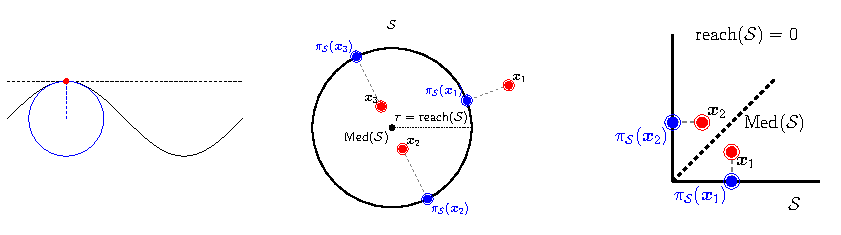
\includegraphics[width=\textwidth]{\toplevelprefix/chapters/appendixB/figs/curvature-fig.pdf}
%
%     \caption{曲率和reach。\textbf{左:}抽象地,曲率可以被认为是量化光滑表面与其局部线性近似的偏差。对于曲线,这方面有一个精确的刻画,即相关圆的“曲率半径”。\textbf{中:}reach根据到集合的投影函数的单射性来定义曲率,使其可以独立于可微性来定义。在$\cS$是圆的情况下,中轴是圆心,reach是圆的半径。\textbf{右:}具有零reach的集合具有某种形式的有缺陷的正则性。例如,‘角’导致零reach。}
%     \label{fig:curvature-reach}
% \end{figure}
%
% \subsection{几何正则性:曲率和Reach}
%
% 对于具有足够光滑(比如可微)的几何结构的集合,正则性可以用\textit{曲率}来理解:集合在其局部线性近似处偏离的速度(\Cref{fig:curvature-reach},左)。在某种意义上,这可以被认为是与实变函数理论中的二阶泰勒近似类似。曲率的研究相当深入,仔细利用它已经导致了一些最长期的数学开放问题的解决(也许最著名的是佩雷尔曼对庞加莱猜想的证明\cite{Perelman2002-bt,Perelman2003-xe,Perelman2003-yk})。
%
% 我们将稍微间接地对支撑集$\cS$施加一个曲率条件,使用一个称为\textit{reach}的量\cite{Federer1959-gk}。这将使我们能够避免对集合$\cS$的平滑性做出明确的假设,因为\Cref{thm:covering-number-rate-distortion}的内容纯粹是用度量量来表述的。我们对这个性质的阐述受到\textcite{Aamari2019-mp}的表述的影响。对于一个(闭)集$\cS \subset \R^D$,考虑到该集合的距离函数:对于任何$\vx \in \R^D$,
% \begin{equation}\label{eq:dist-func}
%     \dist(\vx, \cS) = \inf_{\vx' \in \cS} \norm*{\vx - \vx'}_2.
% \end{equation}
% 对于一个紧集$\cS$,魏尔斯特拉斯定理意味着对于任何$\vx \in \R^D$,总有一些$\vx' \in \cS$在距离函数中达到下确界。reach是根据下确界\textit{唯一}达到的那些点来定义的。定义$\cS$的中轴为
% \begin{equation}
%     \mathrm{Med}(\cS) = \set*{
%         \vx \in \R^D \given \exists \vx' \neq \vx'' \in \cS,
%         \norm*{\vx - \vx'}_2 = \norm*{\vx - \vx''}_2 = \dist(\vx, \cS)
%     },
% \end{equation}
% 这是下确界非唯一达到的点的集合。我们定义reach为
% \begin{equation}
%     \mathrm{reach}(\cS) = \inf_{\vx \in \cS} \dist(\vx, \mathrm{Med}(\cS)).
% \end{equation}
% 中轴可以为空(考虑一个凸集$\cS$),在这种情况下,reach为$+\infty$。如果它不为空,则reach是有限的。它可以被理解为曲率的一个概念(\Cref{fig:curvature-reach},中和右)。我们假设:
% \begin{assumption}\label{assumption:positive-reach}
%     随机变量$\vx$的支撑$\cS \subset \R^D$是紧的,具有正的reach。
% \end{assumption}
%
% \Cref{assumption:positive-reach}对我们的主要后果是,对于\textit{任何}低于reach的点,到集合$\cS$的\textit{投影}可以被唯一定义。更精确地说,如果$\cS$满足$\mathrm{reach}(\cS) = \tau > 0$,那么对于任何$\vx$满足$\dist(\vx, \cS) < \tau$,优化问题
% \begin{equation}
%     \argmin_{\vx' \in \cS}\, \norm*{\vx - \vx'}_2
% \end{equation}
% 有一个唯一的解(通过紧性达到),因此我们可以定义一个投影映射
% \begin{equation}
%     \pi_{\cS}(\vx) \doteq
%     \argmin_{\vx' \in \cS}\, \norm*{\vx - \vx'}_2
% \end{equation}
% 在域$\set{\vx \in \R^D \given \dist(\vx, \cS) < \tau}$上,值域为$\cS$。这个事实将在\Cref{thm:covering-number-rate-distortion}的证明中使用。
%
% 为了避免过度的技术复杂性,我们对支撑集$\cS$做一个额外的简化假设。为了介绍它,我们需要两个在正reach集合理论中基础的额外几何定义。
% 设$\mathrm{tan}(\cS, \vx)$表示$\cS$在点$\vx \in \cS$处的切锥:
% \begin{equation}\label{eq:tangent-cone}
%     \mathrm{tan}(\cS, \vx) = \set*{\vu \in \R^D \mid \exists \vx_i \in \cS, r_i > 0 \::\: r_i(\vx_i - \vx) \to_{i \to \infty} \vx} \cup \set{\Zero}.
% \end{equation}
% 在微分几何中,切空间表示对底层流形的最佳局部线性近似。在正reach集合理论中,前面的定义给出了一个类似但更一般的结构,它不要求可微性。
% $\cS$在$\vx \in \cS$处的法锥是根据切锥定义的:
% \begin{equation}\label{eq:normal-cone}
%     \mathrm{nor}(\cS, \vx) = \set*{\vu \in \R^D \mid \ip{\vu}{\vv} \leq 0,\,
%     \forall \vv \in \mathrm{tan}(\cS, \vx)}.
% \end{equation}
% 在微分几何中,法空间是切空间的正交补——它给出了在给定点(局部地)远离流形的方向集。前面的定义将这个概念推广到非可微集合,为此我们需要考虑切锥而不是切向量空间;对于锥,前面的定义是正交补的适当推广,因为法锥的所有元素与切锥的所有元素至少成$90$度角。
%
% \begin{assumption}\label{assumption:no-boundary}
%     随机变量$\vx$的支撑$\cS \subset \R^D$具有豪斯多夫维数$d$,如果$d \geq 1$,则集合$\cS^{(d-1)} = \set*{\vx \in \cS \given \dim(\mathrm{nor}(\cS, \vx)) \geq D-d+1}$为空。
% \end{assumption}
%
% \Cref{assumption:no-boundary}是技术性的,但可以直观地认为是要求支撑集$\cS$在被视为$\bR^D$的子流形时具有空边界。特别是,当$\cS$是一个没有边界的可微流形时,\Cref{assumption:no-boundary}是满足的,因为在这种情况下,切空间都是相同维数的向量空间。我们不在这里讨论豪斯多夫维数,除了提到它可以被认为是将子空间或流形的维数推广到$\bR^D$的任意子集——更多细节请参见,例如,\cite{Evans1991-pp}。



% \subsection{Proof of
% \texorpdfstring{\Cref{thm:covering-number-rate-distortion}}{Relationship
% Between Rate Distortion and Covering}}
\subsection{率失真与覆盖之间关系的证明}

我们简要地勾勒证明,然后着手建立三个基本引理,然后给出证明。证明将依赖于下面勾勒中介绍的概念。

获得率失真函数\eqref{eqn:rate-distortion-general}的上界是直接的:根据率的刻画(即,率失真函数是$\vx$在期望平方$\ell^2$失真为$\epsilon$的编码的最小率),上界$\cR_{\epsilon}(\x)$只需要证明一个$\x$的编码达到这个目标失真,而$\Supp(\x)$的任何$\epsilon$-覆盖都能达到这个目标,其率等于覆盖基数的以$2$为底的对数。
下界则更为微妙。我们利用香农下界,在\Cref{rem:slb}中讨论过:计算\cite[\S III, (22)]{Linder1994-ej}中的常数给出了\Cref{eq:slb}中引用的结果的更精确版本(当然,以比特为单位):对于任何具有紧支撑和密度函数的随机变量$\vx$,成立
\begin{equation}\label{eq:slb-appendix-1}
    \cR_{\epsilon}(\x)
    \geq
    h(\x)
    - \log \volume(B_{\epsilon})
    +
    \log
    \left(
    \frac{
    	2
    }
    {
    	D \Gamma(D/2)
    }
    \left(
    \frac{
    	D
    }
    {
    	2e
    }
    \right)^{D/2}
    \right),
\end{equation}
此表达式中的熵(等)以奈特为单位。
常数可以很容易地用斯特林近似来估计。
一个通常有用的斯特林近似的定量形式给出对于任何$x > 0$ \cite{Jameson2015-hy}
\begin{equation}
    \Gamma(x) \leq \sqrt{2\pi} x^{x - 1/2} e^{-x} e^{1/(12x)}.
\end{equation}
我们将这个界应用于\Cref{eq:slb-appendix-1}中的$\Gamma(D/2)$。
我们得到
% 由于$D \geq 1$,我们有$e^{1/(6D)} \leq e^{1/6}$,且
\begin{align}
    \log
    \left(
    \frac{
        2
    }
    {
        D \Gamma(D/2)
    }
    \left(
    \frac{
        D
    }
    {
        2e
    }
    \right)^{D/2}
    \right)
    &\geq
    -\frac{1}{6D}
    +
    \log\left(
        \frac{2}{D} 
        \left(
        \frac{
            D
        }
        {
            2e
        }
        \right)^{D/2}
        \cdot
        \sqrt{\frac{D}{4\pi}}
        \left(
        \frac{D}{2e}
        \right)^{-D/2}
    \right)
    \\
    &=
    -\frac{1}{6D}
    - \frac{1}{2}\log D\pi,\label{eq:slb-constant-est}
\end{align}
我们可以将其作为\Cref{eq:slb}中常数$C_D$的显式值。
总结完全量化的香农下界(以比特为单位):
\begin{equation}\label{eq:slb-appendix}
    \cR_{\epsilon}(\x)
    \geq
    h(\x)
    - \log_2 \volume(B_{\epsilon})
    % - \frac{1}{2} \log(D\pi) 
    - O(\log D).
\end{equation}

现在,我们当前目的的重要约束是香农下界要求随机变量$\vx$具有密度函数,这排除了许多感兴趣的低维分布。
但让我们暂时考虑$\vx$确实有密度函数的情况。
$\vx$在其支撑上均匀分布的假设在这种情况下很容易形式化:对于任何波莱尔集$A \subset \cS$,我们有
\begin{equation}
    \Pr[\vx \in A] = \int_{A} \frac{1}{\volume(\cS)} \odif \vx.
\end{equation}
那么熵$h(\vx)$就是
\begin{equation}
    h(\vx) = \log_2 \volume(\cS).
\end{equation}
然后证明以一个引理结束,该引理将比率$\volume(\cS) / \volume(B_{\epsilon})$与$\cS$被$\epsilon$球的$\epsilon$-覆盖数联系起来。
% 更一般地,特别是对于低维分布,我们可以给出$\vx$在其支撑上均匀分布的严格定义,根据\sdb{COMPLETE}


为了将上述程序扩展到满足\Cref{assumption:union-of-spheres}的退化分布,我们对\Cref{thm:covering-number-rate-distortion}中下界的证明将利用一个近似论证,即用“附近的”具有密度函数的低维分布来近似实际的低维分布$\vx$。
% 我们还将确保近似序列是
% 我们将使用\Cref{assumption:positive-reach}来确保这种近似是可能的,并且发生的“收敛”足够正则,以便我们能够根据近似分布的率失真来估计$\vx$的率失真。
然后,我们将近似序列中引入的参数与失真参数$\epsilon$联系起来,以获得\Cref{thm:covering-number-rate-distortion}中期望的结论。


\begin{definition}\label{def:thickening-set}
    设$\cS$是一个紧集。
    % 满足\Cref{assumption:positive-reach}。
    对于任何$\delta > 0$,定义$\cS$的$\delta$-增厚,记为$\cS_{\delta}$,由
    \begin{equation}
        \cS_{\delta} = \set*{\vxi \in \R^D \given \mathrm{dist}(\vxi, \cS) \leq
        \delta}.
    \end{equation}
\end{definition}
\Cref{def:thickening-set}中引用的距离函数由下式定义
\begin{equation}\label{eq:dist-func}
    \dist(\vxi, \cS) = \inf_{\vxi' \in \cS} \norm*{\vxi - \vxi'}_2.
\end{equation}
对于一个紧集$\cS$,魏尔斯特拉斯定理意味着对于任何$\vxi \in \R^D$,总有一些$\vxi' \in \cS$在距离函数中达到下确界。
% \eqref{eq:dist-func},及其随后讨论的性质。
$\cS_{\delta}$的紧性很容易从$\cS$的紧性得出,所以对于任何$\delta > 0$,$\volume(\cS_{\delta})$是有限的。然后可以对增厚随机变量做出以下定义,专门针对\Cref{assumption:union-of-spheres}。

% \begin{definition}\label{def:thickening-rv}
%     设$\vx$是一个随机变量,使得$\Supp(\vx) = \cS$是紧的。
%     定义增厚随机变量$\vx_{\delta}$为在集合$\cS_{\delta}$上均匀分布(\Cref{def:thickening-set})。
% \end{definition}

\begin{definition}\label{def:thickening-rv-uos}
    设$\vx$是一个随机变量,使得$\Supp(\vx) = \cS$是$K$个超球面的并集,如\Cref{assumption:union-of-spheres}中所述分布。
    将混合的每个分量的支撑表示为$\cS_k$。
    定义增厚随机变量$\vx_{\delta}$为测度的混合,其中每个分量测度在增厚集$\cS_{k, \delta}$上均匀(\Cref{def:thickening-set}),对于$k \in [K]$,混合权重为$\pi_k$。
\end{definition}


\begin{lemma}\label{lem:rate-distortion-lb-uos}
    假设随机变量$\vx$满足\Cref{assumption:union-of-spheres}。那么如果$0 < \delta < \tfrac{1}{2}$,增厚随机变量$\vx_{\delta}$(\Cref{def:thickening-rv-uos})对于任何$\epsilon > 0$满足
    \begin{equation}
        R_{\delta + \epsilon}(\vx_{\delta})
        \leq
        R_{\epsilon}(\vx).
    \end{equation}
\end{lemma}

\Cref{lem:rate-distortion-lb-uos}的证明推迟到\Cref{sec:app-rate-dist-deferred-proofs}。
使用\Cref{lem:rate-distortion-lb-uos},上述程序可以实现,因为随机变量$\vx_{\delta}$具有相对于勒贝格测度均匀的密度。

\begin{proof}[(Proof of \Cref{thm:covering-number-rate-distortion})]
    上界很容易证明。如果$S$是$\vx$支撑的任何$\epsilon$-覆盖,其基数为$\cN_{\epsilon}(\Supp(\vx))$,那么考虑将每个$\vxi \in \Supp(\vx)$分配给重构$\hat{\vxi} = \argmin_{\vxi' \in S}\, \norm{\vxi - \vxi'}_2$的编码方案,平局任意打破。那么平局发生的概率为零,并且$S$以尺度$\epsilon$覆盖$\Supp(\vx)$的事实保证了失真不大于$\epsilon$;该方案的率为$\log_2 \cN_{\epsilon}(\Supp(\vx))$。

    对于下界,设$0 < \delta < \tfrac{1}{2}$,并考虑增厚随机变量$\vx_{\delta}$。根据\Cref{lem:rate-distortion-lb-uos},我们有
    \begin{equation}
        R_{\delta + \epsilon}(\vx_{\delta})
        \leq
        R_{\epsilon}(\vx).
    \end{equation}
    由于$\vx_{\delta}$具有均匀的勒贝格密度,我们可以应用香农下界,形式为\eqref{eq:slb-appendix},得到
    \begin{equation}\label{eq:slb-proof}
        % h(\x)
        \log_2 \volume(\Supp(\vx_{\delta}))
        - \log_2 \volume(B_{\delta + \epsilon})
        - O(\log D)
        \leq
        R_{\epsilon}(\vx).
        % R_{\sqrt{2(\delta^2 + \epsilon^2)}}(\vx_{\delta}).
    \end{equation}
    最后,我们需要下界比率
    \begin{equation}
        \frac{
            \volume(\Supp(\vx_{\delta}))
        }
        {
            \volume(B_{\delta + \epsilon})
        }
    \end{equation}
    用覆盖数来表示。
    由于$\Supp(\vx_{\delta}) = \Supp(\vx) + B_{\delta}$,其中$+$在这里表示闵可夫斯基和,体积界论证的一个标准应用(参见例如\cite[命题 4.2.12]{Vershynin2018-br})给出
    \begin{equation}
        \volume(\Supp(\vx_{\delta}))
        \geq
        \cN_{2\delta}(\Supp(\vx))
        \volume(B_{\delta}).
    \end{equation}
    因此
    \begin{align}
        \frac{
            \volume(\Supp(\vx_{\delta}))
        }
        {
            \volume(B_{\delta + \epsilon})
        }
        &\geq
        \cN_{2\delta}(\Supp(\vx))
        \frac{
            \volume(B_{\delta})
        }
        {
            \volume(B_{\delta + \epsilon})
        }
        \\
        &=
        \cN_{2\delta}(\Supp(\vx))
        \left(
            \frac{
                \delta
            } 
            {
                \delta + \epsilon
            }
        \right)^D.
    \end{align}
    选择$\delta = \epsilon / 2$从香农下界\eqref{eq:slb-proof}和上述估计中得到
    \begin{equation}
        \log_2 \cN_{\epsilon}(\Supp(\vx))
        - O(D)
        \leq
        R_{\epsilon}(\vx),
    \end{equation}
    这正是要证明的。

\end{proof}



\subsection{引理\ref{lem:rate-distortion-lb-uos}的证明}\label{sec:app-rate-dist-deferred-proofs}

\begin{proof}[(Proof of \Cref{lem:rate-distortion-lb-uos})]
    只需证明任何期望平方失真为$\epsilon^2$的$\vx$编码都会产生一个具有相同率且失真不会大很多的$\vx_{\delta}$编码,对于合适的$\delta$选择。
    因此,固定一个这样的$\vx$编码,达到率$R$和期望平方失真$\epsilon^2$。我们用$\hat{\vx}$表示使用此编码重构的随机变量,用$\mathrm{q} : \Supp(\vx) \to \Supp(\vx)$表示相关的编码-解码映射(即$\hat{\vx} = \mathrm{q}(\vx)$)。

    现在设$\cS_k$表示$\vx$支撑中的第$k$个超球面。存在一个正交基$\vU_{k} \in \R^{D \times d_k}$使得$\Span(\cS_k) = \Span(\vU_k)$。
    支撑集$\cS$的以下正交分解将在整个证明中重复使用。
    我们有
    \begin{align}
        \cS_{\delta} 
        &= \set{\vxi \in \R^D \given \exists k \in [K] \::\: \dist(\vxi,
        \cS_k) \leq \delta}
        \\
        &= \bigcup_{k \in [K]} \set{\vxi \in \R^D \given \dist(\vxi,
        \cS_k) \leq \delta}.
    \end{align}
    通过正交投影,对于任何$k \in [K]$,任何$\vxi \in \R^D$都可以写成$\vxi = \vxi^{\|} + \vxi^{\perp}$,其中$\vxi^{\|} \in \Span(\cS_k)$且$\ip{\vxi^{\|}}{\vxi^\perp} = 0$。
    那么对于任何$\vxi' \in \cS_k$,我们有
    \begin{align}
        \norm*{\vxi - \vxi'}_2^2 
        = 
        \norm*{\vxi^{\|} + \vxi^{\perp} - \vxi'}_2^2
        &=
        \norm*{\vxi^{\|}}_2^2 + \norm*{\vxi^{\perp}}_2^2 + \norm*{\vxi'}_2^2
        - 2 \ip*{\vxi^{\|}}{\vxi'}
        \\
        &\geq
        \norm*{\vxi^{\|}}_2^2 + \norm*{\vxi'}_2^2
        - 2 \ip*{\vxi^{\|}}{\vxi'}
        \\
        &=
        \norm*{\vxi^{\|} - \vxi'}_2^2.
    \end{align}
    此外,已知对于任何非零$\vxi^{\|} \in \Span(\cS_k)$,
    \begin{equation}
        \inf_{\vxi' \in \cS_k}\,
        \norm*{\vxi^{\|} - \vxi'}_2^2
        =
        \norm*{\vxi^{\|} - \frac{\vxi^{\|}}{\norm{\vxi^{\|}}_2}}_2^2.
    \end{equation}
    如果$\vxi^{\|}$为零,很明显对于每个$\vxi' \in \cS_k$,上述距离等于$1$。
    因此,如果我们定义一个投影映射$\pi_{\cS_k}(\vxi)$为
    \begin{equation}
        \pi_{S_k}(\vxi) = \frac{\vU_k\vU_k^\top \vxi}{\norm{\vU_k^\top \vxi}_2}
    \end{equation}
    对于任何$\vxi \in \R^D$且$\vU_k^\top \vxi \neq \mathbf{0}$,那么$\pi_{\cS_k}(\vxi) = \argmin_{\vxi' \in \cS_k}\norm*{\vxi' - \vxi}_2$。
    我们选择$0 < \delta < 1$,这样增厚集$\cS_{\delta}$不包含任何使得投影映射$\pi_{\cS_k}$未良定义的点$\vxi \in \R^D$。
    所以增厚集$\cS_{\delta}$满足
    \begin{align}
        \cS_{\delta} 
        &= \bigcup_{k \in [K]} \set*{\vxi \in \R^D \given 
        \norm*{\vxi - \frac{\vU_k\vU_k^\top \vxi}{\norm{\vU_k^\top \vxi}_2}}_2
        \leq \delta}.
    \end{align}
    这些距离可以用正交分解重写为
    \begin{align}
        \norm*{\vxi - \frac{\vU_k\vU_k^\top \vxi}{\norm{\vU_k^\top \vxi}_2}}_2^2
        &=
        \norm*{\vxi}_2^2 - 2 \norm{\vU_k^\top \vxi}_2 + 1
        \\
        &=
        \norm*{\vxi^{\|}}_2^2 
        + \norm*{\vxi^{\perp}}_2^2
        - 2 \norm{\vU_k^\top \vxi^{\|}}_2 + 1
        \\
        &=
        \norm*{\vxi^{\perp}}_2^2
        + \left( \norm*{\vxi^{\|}}_2 - 1 \right)^2.
        \label{eq:distance-to-hypersphere}
    \end{align}
    我们接下来要证明,每个这样的$\vxi \in \cS_{\delta}$都可以唯一地与混合中单个子空间的投影相关联,这将允许我们定义一个到$\cS$的相应投影。
    给定一个$\vxi \in \cS_{\delta}$,根据上述,我们可以找到一个子空间$\vU_k$,使得正交分解$\vxi = \vxi^{\|}_k + \vxi^{\perp}_k$满足
    \begin{equation}
        \norm*{\vxi^{\perp}_k}_2^2
        + \left( \norm*{\vxi^{\|}_k}_2 - 1 \right)^2
        \leq
        \delta^2.
    \end{equation}
    考虑对于某个$j \neq k$的分解$\vxi = \vxi_j^{\|} + \vxi_j^{\perp}$。我们有
    \begin{align}
        \norm*{\vxi_j^{\|}}_2
        =
        \norm*{
            \vU_j \vU_j^\top \vxi 
        }_2
        &=
        \norm*{
            \vU_j \vU_j^\top( \vU_k \vU_k^\top \vxi + (\vI - \vU_k \vU_k^\top)
            \vxi )
        }_2
        \\
        &=
        \norm*{
            \vU_j \vU_j^\top (\vI - \vU_k \vU_k^\top) \vxi
        }_2
        \\
        &\leq
        \norm*{
            (\vI - \vU_k \vU_k^\top) \vxi
        }_2
        =
        \norm*{
            \vxi_k^{\perp}
        }_2
        \leq \delta,
    \end{align}
    其中第二行使用了子空间$\vU_k$的正交性假设,第三行使用了正交投影是非扩张的这一事实。
    因此,第$j$个距离满足
    \begin{equation}
        \norm*{\vxi^{\perp}_j}_2^2
        + \left( \norm*{\vxi^{\|}_j}_2 - 1 \right)^2
        \geq
        (1 - \delta)^2.
    \end{equation}
    这意味着如果$0 < \delta < 1/2$,每个$\vxi \in \cS_{\delta}$在混合中都有一个唯一的最近子空间。
    因此,在此条件下,以下映射$\pi_{\cS} : \cS_{\delta} \to \cS$是良定义的:
    \begin{equation}
        \pi_{\cS}(\vxi) 
        =
        \pi_{\cS_{k_\star}}(\vxi),
        \enspace\text{其中}\enspace
        k_{\star} = \argmin_{k \in [K]}\,
        \dist(\vxi, \cS_{k}).
    \end{equation}

    % 同样地,我们有最优性条件
    % \begin{equation}
    %     \vxi = \pi_{\cS_k}(\vxi)
    %     \iff
    %     \vxi = \vU_k \vz
    %     \enspace \text{对于某个} \enspace
    %     \vz \in \R^{d_k} \::\: \norm{\vz}_2 = 1.
    % \end{equation}
    % 因此,对于任何$\vxi \in \cS_{\delta}$,我们可以写成$\vxi = \vU_k \vz + \veps$,对于某个$k \in [K]$,某个$\norm{\vz}_2 = 1$和某个$\norm{\veps}_2 \leq \delta$。
    %     给定表示$\vxi = \vU_k \vz + \veps$,
    % 注意到
    % \begin{equation}
    %     \dist(\vxi, \cS_k) = 
    % \end{equation}
    %
    % 这意味着不可能有$\vxi \in \cS_{\delta}$和$k \neq k'$使得
    % $\pi_{\cS_k}(\vxi) = \vxi$和
    % $\pi_{\cS_{k'}}(\vxi) = \vxi$。因为如果这是真的,我们将有$\vU_k
    % \vz = \vU_{k'} \vz'$对于某个单位范数$\vz, \vz'$,根据最优性条件,这与子空间$\vU_k$的假定相互正交性相矛盾。
    % 此外,从假定的条件$\sum_{k\in [K]} d_k = D$和每个$\vU_k$的相互正交性可以得出,对于任何$\vxi \in \R^D$,存在

    现在,我们通过以下方式为$\vx_{\delta}$定义一个编码
    \begin{equation}
        \hat{\vx}_{\delta} = \mathrm{q}( \pi_{\cS}(\vx_{\delta}) ).
    \end{equation}
    显然,这与一个率-$R$的$\vx_{\delta}$编码相关联,因为它使用了$\vx$的率-$R$编码的编码-解码映射。我们必须证明它达到了小的失真。
    我们计算
    \begin{align}
        \bE\left[ \norm*{ \vx_{\delta} - \hat{\vx}_{\delta} }_2^2 \right]
        &=
        \bE\left[ \norm*{ \vx_{\delta} - \mathrm{q}(\pi_{\cS}(\vx_{\delta})) }_2^2 \right]
        \\
        &\leq
        \left(
        \bE\left[ \norm*{ \vx_{\delta} - \pi_{\cS}(\vx_{\delta}) }_2^2
        \right]^{1/2}
        + \bE\left[ \norm*{ \pi_{\cS}(\vx_{\delta})
        - \mathrm{q}(\pi_{\cS}(\vx_{\delta})) }_2^2 \right]^{1/2}
        \right)^2,\label{eq:distortion-decomposition}
    \end{align}
    其中不等式使用了闵可夫斯基不等式。
    现在,根据\Cref{def:thickening-set,def:thickening-rv-uos},我们确定性地有
    \begin{equation}
        \norm*{ \vx_{\delta} - \pi_{\cS}(\vx_{\delta}) }_2^2
        \leq \delta^2,
    \end{equation}
    所以期望也满足这个估计。
    对于第二项,只需刻画随机变量$\pi_{\cS}(\vx_{\delta})$的密度与$\vx$的密度足够接近即可——正如\Cref{assumption:union-of-spheres}所暗示的,$\vx$的密度是每个子球面$\cS_k$上均匀分布的混合。
    根据上面的论证,每个点$\vxi \in \cS_{\delta}$都可以与一个且仅一个子空间$\vU_k$相关联,这意味着$\cS_{\delta}$定义中的混合分量(回顾\Cref{def:thickening-rv-uos})不重叠。因此,$\pi_{\cS}(\vx_{\delta})$的密度可以通过研究$\pi_{\cS_k}$对条件随机变量$\vx_{\delta}$(条件是 从$\cS_{k, \delta}$中抽取)的影响来刻画。将此测度表示为$\mu_{k, \delta}$。
    我们声称此测度在$\pi_{\cS_k}$下的推前测度在$\cS_k$上是均匀的。
    为了看到这一点,我们回顾\Cref{eq:distance-to-hypersphere},它给出了刻画
    \begin{equation}
        \cS_{k, \delta} = \set*{
            \vxi^{\|} + \vxi^{\perp} 
            \given 
            \vxi^{\|} \in \Span(\vU_k),
            \vxi^{\perp} \in \Span(\vU_k)^\perp,
            \norm*{\vxi^{\perp}}_2^2
            + \left( \norm*{\vxi^{\|}}_2 - 1 \right)^2
            \leq
            \delta
        }.
    \end{equation}
    所讨论的条件分布在此集合上是均匀的;我们需要证明应用于此条件随机变量的投影$\pi_{\cS_k}$产生一个在$\cS_k$上均匀的随机变量。
    关于这些坐标,我们已经看到$\pi_{\cS_k}(\vxi^\| + \vxi^\perp) = \vxi^\| / \norm{\vxi^{\|}}_2$。
    因此,对于任何$\vxi \in \cS_{k}$,我们在$\cS_{k, \delta}$中$\vxi$在$\pi_{\cS_k}$下的原像为
    \begin{equation}
        \pi_{\cS_k}^{-1}(\vxi) = \set*{
            r\vxi + \vxi^\perp 
            \given
            r > 0,
            \vxi^{\perp} \in \Span(\vU_k)^\perp,
            \norm*{\vxi^{\perp}}_2^2
            + \left( r - 1 \right)^2
            \leq
            \delta
        }.
        \label{eq:fiber-of-uos}
    \end{equation}
    为了证明$(\pi_{\cS_k})_{\sharp} \mu_{k, \delta}$是均匀的,我们需要以一种方式分解$\cS_{k, \delta}$上均匀密度的积分,使得每个纤维$\pi_{\cS_k}^{-1}(\vxi)$(对于每个$\vxi \in \cS_k$)对积分的“贡献”是相等的。\footnote{更严谨地说,这对应于将$\cS_{k, \delta}$上的均匀密度分解为对应于$\vxi \in \cS_{k}$的正则条件密度,并证明$\vxi$上的相应密度是均匀的。证明清楚地表明这是真的。}
    根据\Cref{def:thickening-rv-uos},我们有
    \begin{equation}
        \volume(\cS_{k, \delta})
        = \iint_{\Span(\vU_k) \times \Span(\vU_k)^\perp} \mathbf{1}_{
            \norm*{\vxi^{\perp}}_2^2
            + \left( \norm*{\vxi^{\|}}_2 - 1 \right)^2
            \leq
            \delta
        }
        \odif \vxi^{\|} \odif \vxi^{\perp}.
    \end{equation}
    特别是,在正交坐标上的积分是可分的。
    设$\odif \vtheta^{d}$表示$\R^d$中半径为$1$的球面上的均匀(哈尔)测度。将$\vxi^{\|}$积分转换为极坐标,我们有
    \begin{equation}
        \volume(\cS_{k, \delta})
        = \int_{[0, \infty)} \int_{\bS^{d_k-1}} \int_{\Span(\vU_k)^\perp} 
        r^{d_k-1}
        \mathbf{1}_{
            \norm*{\vxi^{\perp}}_2^2
            + \left( r - 1 \right)^2
            \leq
            \delta
        }
        \odif r \odif \vtheta^{d_k} \odif \vxi^{\perp}.
    \end{equation}
    与纤维表示\eqref{eq:fiber-of-uos}相比,我们看到我们需要对前述积分的$r$和$\vxi^\perp$分量进行“积分”,以验证推前是均匀的。
    但这很明显,因为前述表达式表明此积分的值与$\vxi^\|$无关——或者,在上下文中等价地,与球面分量$\vtheta^{d_k}$的值无关。

    因此,从上述论证可以得出$\pi_{\cS}(\vx_{\delta})$是均匀的。
    因为关于$\delta$的假设意味着$\vx_{\delta}$分布中的混合分量不重叠,混合权重$\pi_k$在像$\pi_{\cS}(\vx_{\delta})$中也得以保留,特别是,$\pi_{\cS}(\vx_{\delta})$的分布等于$\vx$的分布。
    因此,\Cref{eq:distortion-decomposition}中的第二项满足
    \begin{equation}
        \bE\left[ \norm*{ \pi_{\cS}(\vx_{\delta}) - \mathrm{q}(\pi_{\cS}(\vx_{\delta})) }_2^2 \right]
        =
        \bE\left[ \norm*{ \vx - \mathrm{q}(\vx) }_2^2 \right]
        \leq
        \epsilon^2,
    \end{equation}
    因为$\mathrm{q}$是$\vx$的一个失真为$\epsilon$的编码。

    我们因此证明了假设的率-$R$、(期望平方)失真-$\epsilon^2$的$\vx$编码产生了一个率-$R$、(期望平方)失真为$\delta + \epsilon$的$\vx_{\delta}$编码。
    这建立了
    \begin{equation}
        R_{\delta + \epsilon}(\vx_{\delta})
        \leq
        R_{\epsilon}(\vx),
    \end{equation}
    这正是要证明的。


    % 选择$0 < \delta < \mathrm{reach}(\cS)$,使用\Cref{assumption:positive-reach},使得投影映射$\pi_{\cS} : \cS_{\delta} \to \cS$对于任何这样的$\delta$都是良定义的。
    % 定义重构$\hat{\vx}_{\delta}$为
    % \begin{equation}
    %     \hat{\vx}_{\delta} = \mathrm{q}( \pi_{\cS}(\vx_{\delta}) ).
    % \end{equation}
    % 显然,这与一个率-$R$的$\vx_{\delta}$编码相关联,因为它使用了$\vx$的率-$R$编码的编码-解码映射。我们必须证明它达到了小的失真。
    % 我们计算
    % \begin{align}
    %     \bE\left[ \norm*{ \vx_{\delta} - \hat{\vx}_{\delta} }_2^2 \right]
    %     &=
    %     \bE\left[ \norm*{ \vx_{\delta} - \mathrm{q}(\pi_{\cS}(\vx_{\delta})) }_2^2 \right]
    %     \\
    %     &\leq
    %     2 \left(
    %     \bE\left[ \norm*{ \vx_{\delta} - \pi_{\cS}(\vx_{\delta}) }_2^2 \right]
    %     + \bE\left[ \norm*{ \pi_{\cS}(\vx_{\delta}) - \mathrm{q}(\pi_{\cS}(\vx_{\delta})) }_2^2 \right]
    %     \right),
    % \end{align}
    % 其中不等式使用了柯西-施瓦茨不等式和三角不等式。
    %
    % 现在,根据\Cref{def:thickening-set,def:thickening-rv},我们确定性地有
    % \begin{equation}
    %     \norm*{ \vx_{\delta} - \pi_{\cS}(\vx_{\delta}) }_2^2
    %     \leq \delta^2,
    % \end{equation}
    % 所以期望也满足这个估计。
    %
    % 对于第二项,注意到$\pi_{\cS}(\vx_{\delta})$通过推前构造在$\cS$上诱导了一个分布$\mu_{\delta}$,只需证明这个诱导分布$\mu_{\delta}$与$\vx$的分布$\mu$足够接近,以利用$\mathrm{q}$达到失真$\epsilon^2$的事实来界定这一项。
    % 这个论证是技术性的,使用了$\R^D$的正reach子集的性质。
\end{proof}



% \begin{lemma}\label{lem:thickened-uniform-projected-near-uniform}
%     设$\vx_{\delta}$表示满足\Cref{assumption:no-boundary,assumption:positive-reach}的随机变量$\vx$的$\delta$-增厚(\Cref{def:thickening-rv}),其中$\cS = \Supp(\vx)$且$\delta < \mathrm{reach}(\cS)$。
%     设$\pi_{\cS}$表示到$\cS$的投影,并设$\mu_{\delta}$表示$\vx_{\delta}$的分布在$\pi_{\cS}$下的推前。
%     那么$\mu_{\delta}$承认一个关于$\cS$上$\dim(\cS)$-维豪斯多夫测度的密度,该密度满足
%     \begin{equation}
%         \sdb{均匀性估计}
%     \end{equation}
%
% \end{lemma}
%
% \begin{proof}
%     我们使用共面积公式和满足\Cref{assumption:no-boundary}的正reach集合的一些结构性质,解析地计算$\pi_{\cS}(\vx_{\delta})$的密度。然后我们用reach来估计它,使用正reach集合的曲率估计。
%
%     首先,我们回顾一个关于正reach集合的基本分解引理,由Federer \cite{Federer1959-gk}提出。它断言映射$f : \mathrm{nor}(\cS) \times (0, \delta] \to (\cS_{\delta} \setminus \cS)$,定义为$f(\vxi, \vu, r) = \vxi + r \vu$,是双射和双利普希茨的,其中$\mathrm{nor}(\cS) = \set*{(\vxi, \vu) \in \bR^D \times \bS^{D-1} \given \vxi \in \cS, \vu \in \mathrm{nor}(\cS, \vxi), \norm{\vu}_2 = 1}$是$\cS$的单位法丛(回顾\Cref{eq:normal-cone}中$\cS$在$\vx$处的法锥的定义)\cite[命题 16]{Thale2008-sv}。
%     此外,在\Cref{assumption:no-boundary}下,我们可以以一种有用的方式分解单位法丛$\mathrm{nor}(\cS)$:\cite[注 4.15(4)]{Federer1959-gk}意味着在这个假设下,在每个点$\vxi \in \cS$处的切锥(回顾\Cref{eq:tangent-cone})实际上是一个维数为$d$的向量空间,因此,在每个点处的法锥也是一个向量空间(特别是切锥/空间的直交补),维数为$D-d$。特别是,单位法丛满足$\mathrm{nor}(\cS) = \cS \times \bS^{D-d-1}$\sdb{这不是真的,只是同构,通常会因点而异...}。
%
%     接下来,我们从上述分解中注意到,映射$f$可以表示为$f : \cS \times \bS^{D - d - 1} \times (0, \delta] \to (\cS_{\delta} \setminus \cS)$。对于任何$t \in (0, \delta]$,考虑水平集$\cS(t) = \set{\vxi \in \R^D \mid \dist(\vxi, \cS) = t}$。那么$\cS(t) \subset \cS_{\delta}$,并且对于每个$\vxi' \in \cS(t)$,存在唯一的$(\vxi, \vu) \in \cS \times \bS^{D-d-1}$使得$f(\vxi, \vu, t) = \vxi'$。
%     特别是,根据距离函数和reach的定义,这意味着$\pi_{\cS}(\vxi') = \vxi$。
%     因此,我们可以通过将$\cS_{\delta}$上的积分分解为由映射$f$规定的独立分量来计算$\pi_{\cS}(\vx_{\delta})$的密度。
%
%     直观上,这种分解表明投影分布是完全均匀的,因为在$\vx$的每个点处的法空间都是相同的。
%     为了严格证明这一点,我们注意到与$\mu_{\delta}$相关的密度$p_{\delta}(\vxi)$必须满足
%     \begin{equation}
%         p_{\delta}(\vx) = \bP[ \pi_{\cS}(\vx_{\delta}) = \vxi ].
%     \end{equation}
%     根据上述分解,我们有
%     \begin{equation}
%         \bP[ \pi_{\cS}(\vx_{\delta}) = \vxi ]
%         =
%         \bP[ \dist(\vx_{\delta}, \vxi) \leq \delta ],
%     \end{equation}
%     因为一个点$\vxi' \in \cS_{\delta}$满足$\pi_{\cS}(\vxi') = \vxi$当且仅当$\vxi' = \vxi + \vu r$对于某个$\vu \in \bS^{D-d-1}$和某个$r \in (0, \delta]$,且$\vx_{\delta}$在$\cS_{\delta}$上是均匀的。
%
%
%     应用面积公式,如\cite[\S 3.2]{Thale2008-sv}中所示,我们通过上述简化得到
%     \begin{equation}
%         \cH^{D}(\cS_{\delta})
%         =
%         \iint_{\cS \times \bS^{D-d-1}}
%         % \mathbf{1}_{B}(\vxi)
%         \int_0^\delta
%         \abs{\det Df(\vxi, \vu, r)} \odif r \odif \cH^{D-d-1}(\vu)
%         \cH^{d}(\vxi).
%     \end{equation}
%     $\pi_{\cS}(\vx_{\delta})$的密度可以从这个表达式中提取出来,通过引入一个指示函数并重新排列:
%     \begin{equation}
%         \mu_{\delta}(B)
%         =
%         \frac{1}{
%             \cH^{D}(\cS_{\delta})
%         }
%         \iint_{\cS \times \bS^{D-d-1}}
%         % \int_{\bS^{D-d-1}}
%         \mathbf{1}_{B}(\vxi)
%         \int_0^\delta
%         \abs{\det Df(\vxi, \vu, r)} \odif r \odif \cH^{D-d-1}(\vu)
%         \cH^{d}(\vxi),
%     \end{equation}
%     其中$B \subset \cS$是$\R^D$的一个波莱尔集,这意味着在$\vxi \in \cS$处的密度$p_{\delta}(\vxi)$是
%     \begin{equation}\label{eq:density-expression-mudelta}
%         p_{\delta}(\vxi)
%         =
%         \frac{1}{
%             \cH^{D}(\cS_{\delta})
%         }
%         \int_{\bS^{D-d-1}}
%         \int_0^\delta
%         \abs{\det Df(\vxi, \vu, r)} \odif r \odif \cH^{D-d-1}(\vu).
%     \end{equation}
%     为了证明结果,我们将用reach来获得这个表达式的上下界。
%     我们计算$f$在一点的雅可比矩阵(任意向量的像)为
%     \begin{equation}
%         Df(\vxi, \vu, r)(\Delta \vxi, \Delta \vu, \Delta r)
%         = \Delta \vxi + \vu \Delta r + r \Delta \vu.
%     \end{equation}
%     对于上述积分中的雅可比行列式,只需在$\cS \times \bS^{D-d-1} \times (0, \delta]$的切空间在任意$(\vxi, \vu, r)$对处的正交基中表示雅可比矩阵即可。
%     遵循\cite[p. 563]{Zahle1986-cp}和\cite[p.\ 138]{Thale2008-sv},存在一个正交系统$\vb_i(\vxi, \vu)$,$i = 1, \dots, D-1$,具有相应的主曲率$\kappa_i(\vxi, \vu) > 0$,使得每个$\vb_i(\vxi, \vu)$与$\vu$正交,并且系统
%     \begin{equation}
%         \va_i(\vxi, \vu) = \left(
%         \frac{1}{\sqrt{1 + \kappa_i^2(\vxi, \vu)}} \vb_i(\vxi, \vu),
%         \frac{\kappa_i(\vxi, \vu)}{\sqrt{1 + \kappa_i^2(\vxi, \vu)}} \vb_i(\vxi, \vu)
%         \right)_{i=1}^{D-1}
%     \end{equation}
%     是$\cS \times \bS^{D-d-1}$的切丛的一个正交系统。
%     在此基中表示雅可比矩阵给出
%     \begin{equation*}
%         Df(\vxi, \vu, r)(\va_i(\vxi, \vu), 0)
%         =
%         \frac{1+r\kappa_i(\vxi, \vu)}{\sqrt{1+\kappa_i^2(\vxi,\vu)}} \vb_i(\vxi,
%         \vu),
%     \end{equation*}
%     且$Df(\vxi, \vu, r)(\Zero, 1) = \vu$,所以定义$\vB(\vxi, \vu) \in \R^{D \times (D-1)}$为列为$\vb_i(\vxi, \vu)$的矩阵,$\vD(\vxi,\vu) \in \R^{(D-1)\times (D-1)}$为第$i$个对角线元素为$(1+r\kappa_i(\vxi,\vu))/\sqrt{1+\kappa_i^2(\vxi,\vu)}$的对角矩阵,计算雅可比行列式等价于计算
%     \begin{equation}
%         \begin{bmatrix}
%             \vB\vD & \vu
%         \end{bmatrix}
%         \begin{bmatrix}
%             \vB\vD & \vu
%         \end{bmatrix}^\top.
%     \end{equation}
%     的行列式的平方根。这里,我们注意到$[\vB, \vu]$是一个正交矩阵。所以行列式就是$\abs{\vD}$的行列式。
%     特别是,我们已经证明
%     \begin{equation}\label{eq:jacobian-determinant-reach}
%         \abs{ \det Df(\vxi, \vu, r)}
%         =
%         \prod_{i=1}^{D-1}
%         \abs{1+r\kappa_i(\vxi,\vu)}/\sqrt{1+\kappa_i^2(\vxi,\vu)}.
%     \end{equation}
%
%     我们最后使用它们在\cite{Zahle1986-cp}中的定义来估计这些主曲率。它们可以与对于任何$r \in (0, \delta]$的超曲面$\cS(r)$的主曲率相关联,根据\cite{Federer1959-gk},这是一个具有利普希茨外法向量$\nu_r : \cS(r) \to \bS^{D-1}$的$C^1$流形,因此几乎处处定义了主曲率$\kappa_i^r(\vxi + r \vu )$作为自伴算子$D \nu_r(\vy)$的特征值,对于$\vy = \vxi + r \vu$。
%     这些可以与上面定义的主曲率相关联(见\cite{Zahle1986-cp})
%     \begin{equation}\label{eq:principal-curvatures}
%         \kappa_i^r(\vxi + r \vu ) = \frac{\kappa_i(\vxi, \vu)}{1
%         + r \kappa_i(\vxi, \vu)}.
%     \end{equation}
%     \textit{先验地}特征值$\kappa_i^r(\vxi + r \vu )$是任意实数,但前面的公式意味着一个约束:为了使\eqref{eq:principal-curvatures}对于每个$0 < r \leq \delta < \mathrm{reach}(\cS)$都是良定义的,分母对于这样的$r$不能为零。如果$\kappa_i(\vxi, \vu) < 0$,这要求$1 + r \kappa_i(\vxi, \vu) > 0$对于所有这样的$r$;等价地
%     \begin{equation}
%         \kappa_i(\vxi, \vu) > -\frac{1}{r}.
%     \end{equation}
%     因为这个界的左侧不依赖于$r$,这通过对$\delta < \mathrm{reach}(\cS)$取上确界意味着
%     \begin{equation}\label{eq:principal-curvatures-not-too-neg}
%         \kappa_i(\vxi, \vu) > -\frac{1}{\mathrm{reach}(\cS)}.
%     \end{equation}
%     也很清楚$\kappa_i(\vxi, \vu) = +\infty$是可能的,在这种情况下\eqref{eq:jacobian-determinant-reach}在极限意义上解释。
%     
%     \sdb{这个段落不对,我们可以让它们的大小等于这个吗?符号取决于$\vu$?(或者符号总是负的...?它取决于法线是向外还是向内...)}
%     此外,在我们的设置中,这些主曲率与水平集$\cS(r)$相关联,我们有一个简化,利用了(如上使用映射$f$建立的)$\cS(r) = \cS \times r\bS^{D-d-1}$这一事实。
%     这特别表明,在$\cS(r)$的任何点处的切空间,通过上述分解表示为$\vxi + r \vu$,分解为$\cS$在$\vxi$处的切空间和$r\bS^{D-d-1}$在$r \vu$处的切空间的直和,这不依赖于$r$。
%     因为球面是一个齐性空间,它的主曲率不依赖于$\vu$(例如,\cite{Lee2018-xb});遵循\textcite[\S 1]{Zahle1986-cp}的注,我们计算这$D-d-1$个主曲率$\kappa_i^r(\vxi + r \vu)$为$1/r$,在$\vxi$和$\vu$上一致。然后可以得出相关的极限主曲率满足$\kappa_i(\vxi, \vu) = +\infty$,所以如果我们假设这些是按升序排序的,我们可以将\eqref{eq:jacobian-determinant-reach}表示为
%     \begin{equation}\label{eq:jacobian-determinant-reach-lowdim}
%         \abs{ \det Df(\vxi, \vu, r)}
%         =
%         r^{D-d-1}
%         \prod_{i=1}^{d}
%         \abs{1+r\kappa_i(\vxi,\vu)}/\sqrt{1+\kappa_i^2(\vxi,\vu)}.
%     \end{equation}
%
%     现在我们使用\eqref{eq:principal-curvatures-not-too-neg}来估计\eqref{eq:jacobian-determinant-reach-lowdim}。
%     对于$r>0$,函数$g(x) = (1 + rx)^2 / (1 + x^2)$(通过微积分)在$x=r$和$x=-1/r$处有两个临界点;检查表明,在$x=-1/r$处的临界点是最小值,在$x=r$处是最大值,因为这里的值满足$g(r) = 1 + r^2$和$g(-1/r) = 0$,而且$g(+\infty) = g(-\infty) = r^2$。
%     此外,函数$g$从$x=-1/r$到$x=r$是单调递增的。
%     我们将此应用于\eqref{eq:jacobian-determinant-reach-lowdim},其中主曲率扮演$x$的角色;使用\eqref{eq:principal-curvatures-not-too-neg},我们有对于所有$i \in [d]$,$\vxi$,$\vu$如果$r < \mathrm{reach}(\cS)$
%     \begin{equation}
%         \frac{{\mathrm{reach}(\cS) - r}}{\sqrt{1 + \mathrm{reach}(\cS)^2}}
%         \leq
%         \abs{1+r\kappa_i(\vxi,\vu)}/\sqrt{1+\kappa_i^2(\vxi,\vu)}
%         \leq
%         \sqrt{1 + r^2}.
%     \end{equation}
%
%     % 类似地,我们可以改进下界。
%     % 根据上述,函数$g$从$x=-1/r$到$x=r$是单调递增的,对于$x \geq r$是单调递减的。所以,如果$x \geq -1/2r$,我们有$g(x) \geq r^2 / (1 + 4r^2)$。
%     % 特别是,如果$r < \mathrm{reach}(\cS) / 2$,
%     % 上述界可以改进为
%     % \begin{equation}
%     %     \frac{r}{\sqrt{1 + 4r^2}}
%     %     <
%     %     \abs{1+r\kappa_i(\vxi,\vu)}/\sqrt{1+\kappa_i^2(\vxi,\vu)}
%     %     \leq
%     %     \sqrt{1 + r^2},
%     % \end{equation}
%     % 这可以用平方根的次可加性松弛为
%     % \begin{equation}
%     %     \frac{r}{1 + 2r}
%     %     <
%     %     \abs{1+r\kappa_i(\vxi,\vu)}/\sqrt{1+\kappa_i^2(\vxi,\vu)}
%     %     \leq
%     %     1 + r.
%     % \end{equation}
%
%     因此,我们有雅可比行列式估计(通过\eqref{eq:jacobian-determinant-reach})
%     \begin{equation}
%         \frac{r^{D-1}}{(1 + 2r)^{D-1}}
%         \leq
%         \abs{ \det Df(\vxi, \vu, r)}
%         \leq
%         (1 + r)^{D-1}.
%     \end{equation}
%     因此,我们可以通过\eqref{eq:density-expression-mudelta}来估计$\mu_{\delta}$的密度$p_{\delta}(\vxi)$为
%     \begin{equation}
%         \int_{\bS^{D-d-1}}
%         \int_0^\delta
%         \left( \frac{r}{1 + 2r}\right)^{D-1}
%         \odif r \odif \cH^{D-d-1}(\vu)
%         \leq
%         \cH^{D}(\cS_{\delta})
%         p_{\delta}(\vxi)
%         \leq
%         \int_{\bS^{D-d-1}}
%         \int_0^\delta
%         (1 + r)^{D-1}
%         \odif r \odif \cH^{D-d-1}(\vu)
%     \end{equation}
%     只要$ r < \mathrm{reach}(\cS) / 2$,这里由$\delta < \mathrm{reach}(\cS)/2$隐含。
%     这个界的两边的积分可以分解为关于$r$和$\vu$的独立积分。我们得到
%     \begin{equation}
%         \int_0^\delta
%         \left( \frac{r}{1 + 2r}\right)^{D-1}
%         \odif r
%         \leq
%         \frac{
%             \cH^{D}(\cS_{\delta})
%             p_{\delta}(\vxi)
%         }{
%             \volume(\bS^{D-d-1})
%         }
%         \leq
%         \int_0^\delta
%         (1 + r)^{D-1}
%         \odif r,
%     \end{equation}
%     因此
%     \begin{equation}
%         \int_0^\delta
%         \left( \frac{r}{1 + 2r}\right)^{D-1}
%         \odif r
%         \leq
%         \frac{
%             \cH^{D}(\cS_{\delta})
%             p_{\delta}(\vxi)
%         }{
%             \volume(\bS^{D-d-1})
%         }
%         \leq
%         \frac{1}{D} \left[
%             (1 + \delta)^D - 1
%         \right]
%     \end{equation}
%
%
%
%
%
%
%
%
%
%
%
% \end{proof}
%
% \begin{remark}
%     \Cref{lem:thickened-uniform-projected-near-uniform}的结论对维度$D$的依赖性很差(指数级)。这是因为需要用最坏情况的估计来处理可能的负曲率,正如证明所示。研究证明表明,如果增加所有主曲率都是非负的假设,可以推导出投影增厚随机变量密度的下界,该下界与上界相匹配,从而大大改善了获得的率。
%
%     同样可能的是,指数率,它依赖于$D$,可以改进为$d$,即支撑集$\cS$的豪斯多夫维数,通过对增厚支撑$\cS(t)$,$0 < t \leq \delta < \mathrm{reach}(\cS)$的主曲率进行更精细的分析,考虑到这些是由增厚一个$d$-维集合生成的。
% \end{remark}








\end{document}
